\documentclass[12pt]{report}
\renewcommand{\baselinestretch}{1.5}      % interline spacing
%
% \includeonly{}
%
%			PREAMBOLO
%
%PROF: dal punto di vista latex... vspace dovrebbe essere una eccezione, tu invece lo hai usato per modificare le spaziature tra paragrafi... non è una cosa che avresti dovuto fare.

%PROF: hai usato molto spesso la convenzione di mettere tra singole virgolette parole chiave, nomi funzioni, nomi file, etc... altre volte li hai messi in corsivo, o in monotype... sarebbe stato da uniformare (le virgolette non mi piacciono molto). Io ti ho almeno corretto la virgoletta di apertura (che in latex è da fare diversa da quella di chiusura, altrimenti viene un apostrofo). Vedi tu se riesci e vuoi modificare. Puoi ritrovare i miei interventi cercando la virgoletta di apertura ` 
%probabilmente molto spesso (e anche in casi in cui non hai usato le virgolette) sarebbe stato da usare \texttt o \verb

%PROF: non ne sono sicuro ma credo che tu non abbia messo neanche una virgola in tutto il testo... avevo cominciato qua e là (dove più evidenti a metterle... ma non ho fatto a tempo a fare revisione anche di questo). 

\usepackage[a4paper]{geometry}
\usepackage{amssymb,amsmath,amsthm}
\usepackage{graphicx}
\usepackage{url}
\usepackage{hyperref}
\usepackage{epsfig}
\usepackage[italian]{babel}
\usepackage{tesi}
\usepackage[procnames]{listings}
\usepackage{color}
\usepackage{xcolor}
\usepackage{caption}
\usepackage{upquote} %PROF: per risolvere problemi apostrofi in listings (p.16 e 17)
\graphicspath{ {./Images/} }
%Figure con bordo
\usepackage{float}
\floatstyle{boxed}
\restylefloat{figure}

\usepackage[backend=bibtex]{biblatex}
\addbibresource{Bibliografia.bib}

% per le accentate
\usepackage[utf8]{inputenc}

%
\newtheorem{myteor}{Teorema}[section]
%
\newenvironment{teor}{\begin{myteor}\sl}{\end{myteor}}
%
%
%           TITOLO
%
\begin{document}
\renewcommand{\baselinestretch}{1.4}      % interline spacing

\definecolor{pink}{RGB}{255,0,90}
\definecolor{blue}{RGB}{0,0,113}
\definecolor{red}{RGB}{255,0,0}
\definecolor{green}{RGB}{0,150,0}
\definecolor{l-blue}{RGB}{0,150,150}
\definecolor{yellow}{RGB}{255,255,0}
\definecolor{black}{RGB}{0,0,0}

% Python style for highlighting
\newcommand\pythonstyle{\lstset{
language=Python,
basicstyle=\ttfamily\fontsize{10pt}{10pt}\selectfont,
otherkeywords={self, then},             % Add keywords here
emph={MyClass,__init__},          % Custom highlighting
%identifierstyle=\color{green},
keywordstyle=\color{green},
commentstyle=\color{l-blue},
stringstyle=\color{blue},
frame=tb,                         % Any extra options here
showstringspaces=false,            % 
belowskip=2em,
procnamekeys={def,class},
upquote=true %PROF: vedi commento upquote sopra
}}


\newcommand\outputstyle{\lstset{
basicstyle=\ttfamily\fontsize{10pt}{10pt}\selectfont,
otherkeywords={info},             % Add keywords here
keywordstyle=\color{l-blue},
keywordstyle=[2]\color{yellow},
keywordstyle=[3]\color{green},
keywordstyle=[4]\color{red},
keywords=[2]{warn},
keywords=[3]{ok},
keywords=[4]{fail}
}}

\newcommand\dictstyle{\lstset{
basicstyle=\ttfamily\fontsize{10pt}{10pt}\selectfont,
commentstyle=\color{black},
otherkeywords={03,05,10,floor_name,suffix_regex,name_regexes,csv_headers,edilizia,buildings,rooms,room_cat,easyroom,AUM01,LAB01,SAL04,SPZ01,group_name,description,scope},
keywordstyle=\color{green},
}}


% Python environment
\lstnewenvironment{python}[1][]
{
\pythonstyle
\lstset{#1}
}{}

% Output environment
\lstnewenvironment{outputl}[1][]
{
\outputstyle
\lstset{#1}
}{}

% Dictionary environment
\lstnewenvironment{dict}[1][]
{
\dictstyle
\lstset{#1}
}{}

% Python for external files
\newcommand\pythonexternal[2][]{{
\pythonstyle
\lstinputlisting[#1]{#2}}}

% Python for inline
\newcommand\pythoninline[1]{{\pythonstyle\lstinline!#1!}}

\title{Spazi-Unimi: \\Progettazione e implementazione dell'integrazione e validazione delle diverse fonti di dati edilizi}
\author{Paolo Venturi}
\dept{Corso di Laurea in Informatica} 
\anno{2013-2014}
\matricola{775021}
\relatore{Prof. Carlo Bellettini}
\correlatore{Dr. Matteo Camilli}
%
%        \submitdate{month year in which submitted to GPO}
%		- date LaTeX'd if omitted
%	\copyrightyear{year degree conferred (next year if submitted in Dec.)}
%		- year LaTeX'd (or next year, in December) if omitted
%	\copyrighttrue or \copyrightfalse
%		- produce or don't produce a copyright page (false by default)
%	\figurespagetrue or \figurespagefalse
%		- produce or don't produce a List of Figures page
%		  (false by default)
%	\tablespagetrue or \tablespagefalse
%		- produce or don't produce a List of Tables page
%		  (false by default)
% 
%			DEDICA
%
\beforepreface
\prefacesection{}
        {\hfill \Large {\sl dedicato ai miei genitori Francesco e Donella}}
% 
%			PREFAZIONE
%
%\prefacesection{Prefazione}

%
%			RINGRAZIAMENTI
%
\prefacesection{Ringraziamenti}
{
Innanzitutto vorrei ringraziare i miei compagni di viaggio per quanto riguarda il progetto Spazi-Unimi: Samuel e Diego. Quest'anno passato con voi è sicuramente stato molto duro e stancante ma grazie al vostro aiuto e alla vostra compagnia penso sia anche il più bello tra quelli trascorsi in università.

Un ringraziamento va anche al professor Carlo Bellettini e al mio correlatore il dottor Matteo Camilli che mi hanno permesso di prendere parte allo svolgimento di questo interessantissimo progetto.

Dopodiché vorrei ringraziare i miei genitori: Francesco e Donella. Grazie a loro ho avuto la possibilità di continuare gli studi, in questi anni lontano da casa mi hanno dato un grande appoggio ed anche nei momenti difficili mi hanno sempre lasciato scegliere la strada che reputavo migliore.     
Un ringraziamento va anche a mio fratello Emanuele con il quale ho condiviso tantissime esperienze negli ultimi anni.

Grazie a tutte le persone che sono venute a trovarmi durante i week-end passati a casa, in particolare un grazie di cuore a mia nonna Maria che mi ha sempre incoraggiato. 

Un grosso grazie a tutti gli amici di Malonno (non scrivo i nomi per paura di dimenticare qualcuno): anche se riusciamo a vederci solo il sabato sera mi avete sempre aiutato a divertirmi e a distrarmi dai `problemi' universitari.

Grazie a tutti i coinquilini che ho avuto nel corso di questi cinque anni `milanesi': grazie a voi mi sento molto cresciuto e migliorato rispetto ai primi tempi passati fuori casa.

%PROF: capisco il momento particolare, ma forse potresti limitare i ringraziamenti a apetti legati alla tesi, o all'università... oppure motivare perché il basket lo è stato in questi anni ("perché mi ha permesso di sopravvivere alla tristeza della università.." :-D )
Vorrei ringraziare i ragazzi della WS Basket: grazie a voi ho avuto la possibilità di continuare a praticare lo sport che più amo nonostante fossi lontano dal mio paese.
Siete un gruppo fantastico e spero di riuscire a giocare con voi ancora a lungo.

Un ringraziamento va ai bambini e ragazzi del minibasket dell'US Malonno: nonostante sono ancora alle prime armi come allenatore spero di avervi aiutato nel migliorare le vostre capacità e il vostro spirito di squadra.
Un grazie anche a Marzio che si impegna sempre tantissimo e mi ha dato l'opportunità di iniziare ad allenare: spero di riuscire a trasmettere a tutti i giocatori la mia passione per questo sport.
}
\afterpreface
% 
% 
%			CAPITOLO 1
\chapter{Il progetto Spazi-Unimi}
\label{Spazi-Unimi}

\section{Introduzione al progetto}

Il progetto Spazi-Unimi nasce dall’esigenza degli utenti (studenti, professori, etc.) dell’Università degli Studi di Milano di cercare in modo facile e veloce la posizione delle aule e altri spazi comuni di loro interesse. 
Vista la dislocazione delle sedi universitarie in varie aree della città (e della regione) un nuovo studente o un visitatore può avere serie difficoltà nell’orientarsi: da qui l’idea di creare una App che semplifichi la ricerca degli edifici universitari e delle loro stanze. 

Spazi-Unimi è stato ideato nell’ambito del progetto Campus Sostenibile\footnote{\url{http://www.campus-sostenibile.unimi.it}}, una collaborazione tra il Politecnico di Milano e l’Università degli Studi di Milano, che si propone di trasformare il quartiere Città Studi in un modello per quanto riguarda la qualità della vita e la sostenibilità.
Dalla proposta del Prof. Carlo Bellettini è quindi partito lo sviluppo del progetto che è stato portato avanti con altri due studenti del dipartimento di Informatica: Samuel Gomes Brandão e Diego Costantino.

\vspace{5mm} %5mm vertical space

I file da cui estrarre le informazioni utili alla creazione dell'applicazione sono stati forniti da due diverse fonti:
\begin{itemize}
\item la Divisione Manutenzione edilizia e impiantistica che ha concesso le piantine delle sedi universitarie e le informazioni sulle aule didattiche;
\item la Divisione sistemi informativi che ha concesso le informazioni sulle aule presenti sul sistema EasyRoom\footnote{\url{http://easystaff.divsi.unimi.it/EasyRoom/index.php}}.
\end{itemize}

\vspace{5mm} %5mm vertical space

Durante le 18 settimane di tirocinio interno al dipartimento di Informatica il lavoro effettuato ha riguardato principalmente lo sviluppo della parte back-end\footnote{Con il termine back-end in questo caso si intende la parte del sistema nascosta all'utente finale il quale interagisce con il front-end cioè l'applicazione.} che si propone di fornire agli addetti delle diverse fonti di dati un modo semplice e immediato per aggiornare le informazioni.
La parte su cui più si è incentrato il mio lavoro è stata l'unione dei dati provenienti dalle diverse fonti cercando di rendere disponibili all'utente finale le migliori informazioni per quanto riguarda completezza e qualità.

Nell'ultima parte del tirocinio invece ci si è concentrati sulla generazione di piantine interattive utili alla futura applicazione multi-piattaforma che costituisce lo scopo finale del progetto Spazi-Unimi.


\newpage
\section{Il problema e i dati forniti per risolverlo}

La prima attività svolta è stato uno studio di fattibilità: sapendo che sul mercato non era presente nessuna applicazione/tool simile a quella che si voleva sviluppare ci si è concentrati più sulla ricerca di possibili librerie utili all'analisi dei file forniti dalle varie fonti. 
Sia l'edilizia che i sistemi informativi hanno fornito dati sulle aule organizzati in fogli elettronici e scritti in formato XLS\footnote{XLS è l'estensione %PROF: prima dici formato e poi estensione (e anche dopo): come informatico non dovresti mischiare questi due concetti. A te della estensione non interessa nulla, qui parli solo di formati
più utilizzata per quanto riguarda i file contenenti fogli di calcolo.}, per quanto riguarda le mappe messe a disposizione dall'edilizia invece le informazioni sono su file di tipo AutoCAD DWG\footnote{DWG (abbreviazione di drawing) è l'estensione principale dei disegni tecnici.}. 

\vspace{5mm} %5mm vertical space

I file XLS essendo per loro natura in formato tabellare risultano di non difficile lettura, ma ancora più semplice risulta quella dei file CSV (Comma-separated values): un formato basato su file di testo ricavabile senza sforzo da fogli elettronici o da database. 

Il formato AutoCAD DWG invece è risultato molto più complicato da analizzare in quanto risulta essere un file binario diviso in diverse sezioni la cui codifica è molto complessa. Vista l'impossibilità di ottenere dati in modo semplice si è cercato un formato più adatto ai nostri scopi in cui esportare la collezione di 606 file DWG forniti. La scelta è ricaduta sull'altro formato AutoCAD cioè il DXF\footnote{DXF (Drawing Interchange Format, o Drawing Exchange Format) estensione di file principalmente utilizzata per l'esportazione su altri sistemi CAD.}: questo standard utilizza un file ASCII diviso in sezioni (HEADER, CLASSES, TABLES, ENTITIES, OBJECTS, THUMBNAILIMAGE ed END OF FILE) risultando quindi facilmente analizzabile tramite un linguaggio di programmazione. La sezione di maggior interesse per in nostri scopi è risultata ENTITIES che contiene tutti gli oggetti disegnati nel file con le loro caratteristiche.

\vspace{5mm} %5mm vertical space

Dimostrata la fattibilità del progetto partendo da questi formati di dati ci si è concentrati sulla ricerca degli scenari d'uso per l'applicazione:        
\begin{itemize}
\item trovare le sedi universitarie vicine alla propria posizione;
\item trovare le stanze di una certa categoria (biblioteche, aule, punti ristoro, etc...) più vicine;
\item cercare le stanze per nome mostrando una lista in caso di ambiguità;
\item mostrare le mappe interne degli edifici rendendole interattive;
\item segnalare errori e problematiche con un apposito form in modo da rendere le informazioni disponibili sempre più corrette e affidabili.
\end{itemize}


\newpage
\section{Scelta di tool, tecnologie e tecniche di sviluppo}

La fase successiva del progetto ha riguardato la scelta delle tecnologie da utilizzare durante lo sviluppo delle funzionalità: prima fra tutte la scelta del linguaggio di programmazione.

Dopo un'esplorazione delle varie possibilità è stato deciso di utilizzare Python\footnote{\url{https://www.python.org}} nella sua ultima versione (la 3). Python è un linguaggio ad alto livello multi-paradigma: è orientato agli oggetti ma possiede caratteristiche dei linguaggi funzionali che rendono molto più semplice e leggibile l'implementazione di alcuni pezzi di codice.

In Python le variabili non sono tipizzate (quindi ogni variabile è un puntatore ad un oggetto): il controllo dei tipi è comunque molto forte e viene fatto tramite tipizzazione dinamica.
Per quanto riguarda la leggibilità del codice in Python viene utilizzata l'indentazione per dividere i programmi in blocchi: ciò porta il codice ad essere molto più elegante rispetto ad altri linguaggi e lo rende molto leggibile anche per chi non conosce il linguaggio.

Gli aspetti funzionali più importanti e più utili alla programmazione presenti in Python sono:
\begin{itemize}
\item le list comprehension, costruttori di liste che utilizzano una modalità di creazione molto intuitiva e matematica;
\begin{python}[title=Esempio di List Comprehension,frame=single]
>>> [(x, y) for x in [1,2,3] for y in [3,1,4] if x != y]
[(1, 3), (1, 4), (2, 3), (2, 1), (2, 4), (3, 1), (3, 4)]
\end{python}

\vspace{5mm} %5mm vertical space
\item i generatori, simili alle list comprehension che non occupano però memoria dato che utilizzano la lazy evaluation\footnote{Con il termine Lazy evaluation si intende una tecnica consistente nel rimandare un'elaborazione finché non verrà realmente richiesta.};
\begin{python}[title=Esempio di Generatore, frame=single]
>>> g=((x, y) for x in [1,2,3] for y in [3,1,4] if x != y)
>>> g
<generator object <genexpr> at 0x7fca9fb91240>
>>> list(g)
[(1, 3), (1, 4), (2, 3), (2, 1), (2, 4), (3, 1), (3, 4)]
\end{python}

\vspace{5mm} %5mm vertical space
\item la parola chiave lambda\footnote{Il nome lambda deriva dal Lambda calcolo cioè un modello di computazione progettato da Alonzo Church e considerato il primo linguaggio di programmazione funzionale.}, utile a definire funzioni anonime utilizzate solo in certe zone del codice, in questo modo non serve associare alla procedura un identificativo.
\begin{python}[title=Esempio di utilizzo della lambda, frame=single]
>>> g = lambda x: x**2
>>> print(g(8))
64
\end{python}

\vspace{5mm} %5mm vertical space
\end{itemize}  
 
Un'altra caratteristica che ci ha portato a scegliere Python è il fatto che sia un linguaggio interpretato e che fornisca una REPL\footnote{Per REPL (Read-Eval-Print-Loop) si intende un interprete da riga di comando avanzato.} (bpython\footnote{\url{http://www.bpython-interpreter.org}}) con la quale provare il codice risulta molto semplice e veloce. 

Ultimo vantaggio dell'usare Python, ma dall'elevata importanza, è il fatto che possieda una vasta libreria standard ed esista uno svariato numero di librerie importabili che possono svolgere e implementare molte funzionalità e algoritmi.

\vspace{5mm} %5mm vertical space

La seconda scelta da effettuare in ambito tecnologico è stata la tipologia di database: vista la grande mole di dati e la loro non completezza si è deciso di utilizzare MongoDB\footnote{\url{https://www.mongodb.org}}.
MongoDB è il database NoSQL\footnote{Categoria di software che non utilizzano il modello relazionale.} più diffuso a livello mondiale, la sua tipologia non è relazionale come per i database classici ma si basa sugli oggetti. 
La memorizzazione dei dati viene effettuata su una tipologia particolare di file JSON\footnote{Per JSON (JavaScript Object Notation) si intende un formato di file basati su JavaScript ed utilizzati per lo più in un contesto di scambio di dati.} detti BSON con uno schema dinamico così che i campi che risulterebbero vuoti in un DB SQL qui non esistono. 

Altro vantaggio della scelta di MongoDB sono le prestazioni in lettura e scrittura di Mongo molto buone per dati di grosse dimensioni come quelli su cui abbiamo lavorato. 
Ciò è anche dovuto al fatto che in MongoDB esiste la possibilità, come nei database relazionali più utilizzati, di creare degli indici che velocizzino la ricerca per campi/documenti usati molto spesso nelle query.
Tra gli indici creabili ve ne è uno in particolare che ci è sembrato molto utile per lo sviluppo del nostro progetto: l'indice geospaziale. 
Dovendo lavorare, tra le altre cose, anche sulle coordinate degli edifici universitari la possibilità di creare un indice per poter effettuare query specifiche basate sulle posizioni geospaziali è sembrata un enorme vantaggio.

Per fare lavorare al meglio il linguaggio (Python 3) con il database (MongoDB) abbiamo inoltre esplorato le librerie disponibili: la scelta è ricaduta su PyMongo\footnote{\url{https://api.mongodb.org/python/current}} che permette in modo facile e veloce di connettersi ad un database MongoDB da un codice Python. 
PyMongo inoltre fornisce la possibilità di effettuare ogni operazione possibile (query, inserimenti, creazioni di collection e di indici, etc.) utilizzando un'interfaccia quasi uguale a quella di MongoDB e ciò ha semplificato l'apprendimento  di tale libreria.  

\vspace{5mm} %5mm vertical space
 
Come per ogni progetto di una certa complessità sorge la necessità di utilizzare un sistema di versioning: la scelta è ricaduta su git\footnote{\url{http://git-scm.com}} uno dei più famosi ed utilizzati software di controllo di versione distribuito. 
Oltre alla possibilità di tenere traccia delle modifiche fatte ai file del progetto git permette di dividere il lavoro in branch separati così da poter sviluppare diverse funzionalità in autonomia e senza modificare il progetto centrale (nel branch `master').
I vari branch sono poi unificabili grazie alla procedura di merge. La repository git così creata è stata poi caricata ad un servizio web di hosting specializzato: GitHub\footnote{\url{https://github.com}}; in questo modo i vari elementi del team di sviluppo hanno potuto sempre avere il codice aggiornato alle ultime modifiche.

\vspace{5mm} %5mm vertical space

A questo punto l'esplorazione si è concentrata sui possibili tool/applicazioni utili all'organizzazione del lavoro e alla raccolta di appunti e note.
Per quanto riguarda l'organizzazione è risultato molto utile e semplice da utilizzare Trello\footnote{\url{https://trello.com}}: si tratta di un'applicazione basata su cartelloni (board).  %PROF: forse qui ci stava un accenno a Kanban
Ogni board è diviso in liste ed ogni lista contiene delle tessere (card) ordinabili: indicando un'attività o una funzionalità da implementare su ogni card si ha un quadro generale molto chiaro dello stato del progetto. 
Durante lo sviluppo abbiamo ordinato le liste in base alle priorità che secondo noi possedeva ogni tessera; grazie alla possibilità di assegnare le tessere ai membri del team inoltre il lavoro di organizzazione è risultato facilitato.

L'ultima applicazione utilizzata è stata Evernote\footnote{\url{https://evernote.com}}: utile alla raccolta di note ed appunti è risultata molto utile per salvare resoconti e insiemi di informazioni molto più grandi rispetto a quelli di Trello. 

\vspace{5mm} %5mm vertical space

Come tecniche di sviluppo del software abbiamo cercato di applicare le pratiche dell'Extreme Programming (XP)\cite{XP} utili al nostro caso. XP è una metodologia di sviluppo del software appartenente alla famiglia delle metodologie agili\footnote{\url{http://agilemanifesto.org}} ed è definita da 12 pratiche principali:
\begin{enumerate}
\item Planning game
\item Brevi cicli di rilascio
\item Uso di una metafora
\item Semplicità di progetto
\item Testing
\item Refactoring
\item Programmazione a coppie 
\item Proprietà collettiva 
\item Integrazione continua
\item Settimana di 40 ore
\item Cliente sul posto
\item Standard di codifica
\end{enumerate}

Il planning game cioè la definizione delle funzionalità da implementare viste le priorità, le stime dei costi e altre valutazione tecniche è stato messo in atto anche grazie all'utilizzo di Trello. 

Il testing è risultato un'importante risorsa nel corso dello sviluppo del progetto: oltre a dare maggiore sicurezza sulla correttezza del codice scritto in molte occasioni è stato utilizzato il TDD. Il TDD (Test Driven Development) è una tecnica utile a guidare la ricerca di un design semplice e efficace, ma ha anche il side-effect di aumentare l'uso dei test e il loro uso come test di non regressione. Lo sviluppo guidato dai test si divide in tre fasi fondamentali:
\begin{itemize}
\item scrittura del test, il test viene scritto in base alla funzionalità che si vuole implementare e deve fallire in quanto tale funzionalità non esiste ancora;
\item implementazione della funzionalità, viene implementato il codice e si controlla tramite il test la sua correttezza; %PROF: la definizione viene fatta tramite il test...
\item refactoring, viene modificato il codice in modo da renderlo più efficiente, leggibile e riusabile.
\end{itemize}

Non sempre però è stato possibile definire dei test in quanto certe funzionalità dipendevano totalmente da librerie esterne o definivano algoritmi procedurali il cui funzionamento era difficilmente testabile in maniera efficace.
In alcuni casi si è cercato di utilizzare il mocking\footnote{Con Mocking si intende una tecnica utile a simulare il comportamento di un oggetto in modo da poter controllare le chiamate su di esso.}, in altri casi la difficoltà nel testare ha portato ad un refactoring della funzionalità mentre nei casi peggiori il test non è stato implementato dato sarebbe stato talmente veicolato da non risultare più utile. 

Oltre ad essere presente nell'approccio TDD il refactoring è stato utilizzato largamente durante lo sviluppo del progetto soprattutto per rendere il codice, non sempre di facile comprensione, il più leggibile ed elegante possibile.

La programmazione a coppie suggerita da Extreme Programming è stata applicata per gran parte del processo di sviluppo nonostante il team fosse composto da 3 elementi. Per ovviare a questo `problema' la composizione della coppia che portava avanti l'implementazione è stata decisa a rotazione: due persone scrivevano codice e una studiava nuove funzionalità o migliorava la propria conoscenza delle tecnologie utilizzate. Soprattutto nella prima parte di sviluppo questo approccio è risultato molto produttivo in quanto tutte le persone del progetto erano alle prime esperienze per quanto riguarda l'uso del linguaggio di programmazione scelto (Python), del database (MongoDB), ma anche per il lavoro in team. Nella seconda parte del progetto invece l'elemento che restava da solo avendo ormai acquisito sufficiente padronanza delle tecnologie scelte poteva sviluppare autonomamente nuove funzionalità.

Lo standard di codifica è stato scelto sempre in funzione della leggibilità e dell'eleganza del codice; il pair programmming inoltre ha aiutato enormemente nel rispettarlo. Per quanto riguarda la documentazione invece si è cercato di aggiungere dei commenti all'inizio di ogni metodo complesso che specificassero la funzione, i parametri in ingresso e i risultati ritornati. Altri commenti invece sono stati inseriti nella parti di codice considerate poco leggibili in modo da aiutare anche un membro esterno al team alla comprensione.   

\newpage
\section{Estrazione dei dati dai file DXF}

La prima parte del progetto Spazi-Unimi ad essere stata sviluppata è quella riguardante la lettura e l'elaborazione delle informazioni estraibili dalle piantine delle sedi universitarie. Come già detto il formato DWG non risultando idoneo ad essere analizzato è stato convertito in un formato DXF grazie all'applicazione free: Teigha® File Converter\footnote{\url{http://www.opendesign.com/guestfiles/teighafileconverter}}. 
Successivamente si è passati all'esplorazione delle librerie Python in grado di leggere tale formato: la scelta è ricaduta sulla libreria dxfgrabber\footnote{\url{http://dxfgrabber.readthedocs.org/en/latest}}. Grazie alla funzione \textit{readfile} di tale libreria si può leggere il contenuto di un file DXF (in qualsiasi versione) e salvarlo in una variabile.
\begin{python}[title=Lettura di un file DXF con dxfgrabber, frame=single]
>>> dxf = dxfgrabber.readfile("File.dxf")
>>> dxf
<dxfgrabber.drawing.Drawing object at 0x7f72d5eef898>
\end{python}

\vspace{5mm} %5mm vertical space

Tale oggetto rispecchia la struttura dei file DXF quindi a noi è bastato leggere la sezione ENTITIES la quale contiene gli oggetti disegnati in tale file.
\begin{python}[title=Salvataggio delle entità di un file DXF, frame=single]
>>> entities = dxf.entities
>>> entities
<dxfgrabber.entitysection.EntitySection object at 0x7f72d608b550>
>>> len(entities)
7850
\end{python}

\vspace{5mm} %5mm vertical space

Come si può notare dal codice preso come esempio ogni piantina contiene migliaia di entità e non tutte sono utili agli scopi del progetto. La scrematura di tali entità è stata fatta grazie ad una caratteristica comune dei disegni CAD: la suddivisione di tali entità in gruppi detti layer. Ogni layer dei file DXF forniti rappresenta un tipo di oggetto ben distinto; dopo un'attenta analisi di tali layer sono stati isolati i più utili:
\begin{itemize}
\item `RM\$', in esso sono contenuti i contorni delle stanze salvati come Polyline (o nella variante LWPolyline);
\begin{python}[title=Analisi del layer `RM\$', frame=single]
>>> rm = [e for e  in entities if e.layer == "RM$"]
>>> rm[0]
<dxfgrabber.entities.Polyline object at 0x7f72d346f9e8>
\end{python}

\vspace{5mm} %5mm vertical space

\item `NLOCALI', contiene le etichette con il codice identificativo di ogni stanza memorizzate come Text (o MText) e linee (per il contorno dei testi);
\begin{python}[title=Analisi del layer `NLOCALI', frame=single]
>>> nloc = [e for e  in entities if e.layer == "NLOCALI" 
            and e.dxftype in ["TEXT", "MTEXT"]]
>>> nloc[0]
<dxfgrabber.entities.Text object at 0x7f72d4afa198>
\end{python}

\vspace{5mm} %5mm vertical space

\item `RM\$TXT', contiene le etichette con il codice identificativo di ogni stanza, la categoria di appartenenza di tale stanza e altre info utili alla Divisione Manutenzione edilizia e impiantistica come la metratura, in questo caso le etichette sono solo di tipo Text (o MText).
\begin{python}[title=Analisi del layer `RM\$TXT', frame=single]
>>> txt = [e for e  in entities if e.layer == "RM$TXT"]
>>> txt[0]
<dxfgrabber.entities.Text object at 0x7f72d345b400>
\end{python}

\vspace{5mm} %5mm vertical space

\end{itemize}

Una volta capito come analizzare e salvare le entità di nostro interesse è stato necessario creare delle classi (nel package `model') che rappresentassero queste entità e che fornissero dei metodi utili per trasformarle. 
La prima classe definita è stata la base per le altre e trattandosi di rappresentare oggetti disegnabili non poteva che essere Point. 
Un oggetto Point è creabile passando due numeri (interi o float) che rappresentano le coordinate sul piano cartesiano di tale punto. 
In tale classe sono stati poi implementati dei metodi di trasformazione utili a dei punti come: traslazione e applicazione di un fattore di scala.

Il passo successivo è consistito nel definire altre tipologie di oggetti che rispecchiassero i dati utili letti dalle entità dei DXF; le classi create sono state:
\begin{itemize}
\item Polygon, definibile come una collezione di punti ordinata che collegati formano un poligono;
\item Text, un testo con un punto che indica la posizione in cui deve essere posto.
\end{itemize}

Analizzando la struttura di tali classi ci si è resi conto che si sarebbero potute rappresentare come oggetti con un punto di ancoraggio: per il testo il punto di posizione mentre per il poligono l'origine. 
Scegliendo però un punto che non fosse l'origine e relativizzando i Point che definiscono un Polygon si possono effettuare certe trasformazioni in maniera molto più semplice. Si è quindi definito un `anchor\_point' per ogni poligono calcolabile come il punto più in basso e più a sinistra del più piccolo rettangolo contenente il poligono (bounding box). 
In questo modo la traslazione di un Polygon si applica solo traslando il suo anchor\_point senza andare a modificare tutti i punti che lo compongono. 
L'evoluzione naturale è stata la definizione di una classe Anchorable dalla quale Polygon e Text ereditano: in questo modo tutti i metodi che implementano le trasformazioni sugli anchor\_point di un oggetto sono definiti nello stesso luogo.

Definite le classi per gli oggetti base si è passati all'implementazione di classi che contenessero tali oggetti: la prima e basilare è Room.
Un oggetto di tipo Room ha il compito di astrarre ciò che definisce una stanza quindi sarà composto da:
\begin{itemize}
\item un oggetto di tipo Polygon che rappresenti il contorno di tale stanza;
\item uno o più oggetti di tipo Text che indichino il contenuto delle etichette associate a tale stanza;
\item un Point che rappresenta il punto di ancoraggio di tale Room in modo da relativizzare tutti gli altri punti della stanza.
\end{itemize}

Giunti a questo punto però ci si è resi conto che Polygon e Room rispetto agli altri tipi di oggetti definiti avevano una particolarità: essendo bidimensionali erano gli unici a poter essere disegnati.
Il passo successivo è stato definire la classe Drawable da cui i poligoni e le stanze potessero ereditare metodi comuni come le trasformazioni e il calcolo del bounding\_box.
I metodi di trasformazione sugli oggetti Drawable non vengono effettuati direttamente: lasciando la responsabilità alle singole classi viene richiamata la trasformazione corrispondente su ogni entità appartenente agli oggetti da modificare.

L'ultima classe del package `model' definita prima dell'effettiva lettura dei file DXF è stata Floor. Un'istanza di tale classe rappresenta un piano di un edificio e come tale oltre ad essere una collezione di Room deve possedere anche informazioni sull'edificio a cui appartiene e sul piano che rappresenta.

Tutte le classi definite in `model' possiedono due metodi particolari:
\begin{itemize}
\item \textit{to\_serializable()}, metodo di istanza che ritorna un dizionario rappresentante l'oggetto su cui è stato richiamato il metodo, tale dizionario può venire memorizzato in un file testuale di tipo JSON;
\item \textit{from\_serializable(dict)}, riceve un dizionario e da esso crea un'istanza della classe usando le informazioni contenute.
\end{itemize}

Per tali metodi inoltre deve valere la seguente proprietà: il risultato dell'applicazione in sequenza dei due metodi su di un oggetto porta alla creazione di un nuovo oggetto uguale a quello di partenza.
In pratica passando un dizionario a \textit{from\_serializable} e applicando al risultato \textit{to\_serializable} si ottiene un dizionario uguale a quello iniziale (stessa cosa con l'ordine dei metodi invertito se si parte da un oggetto di `model'). %PROF: sicuro che debba valere? vuol dire che gli oggetti sono sempre in forma canonica?

\vspace{5mm} %5mm vertical space

Il passo successivo è stato definire una classe DXFReader in grado di leggere i dati da un file DXF e creare un Floor contenente tutti i dati utili.
Dopo aver letto il file con dxfgrabber come visto in precedenza viene richiamata una funzione (\textit{\_extract\_entities()}) %PROF: sicuro dell'undercsore iniziale? non mi pare che adottaste questa convenzione.
che scorre la lista di entità lette e controlla se appartengono alla tipologia e ai layer di nostro interesse.
I testi trovati vengono salvati in un'apposita lista mentre per quanto riguarda le polyline delle stanze vengono sottoposte ad alcune operazioni prima di venire immagazzinate:
\begin{itemize}
\item viene creato un oggetto di tipo Polygon con i punti della polyline trovata;
\item viene controllato che il poligono sia chiuso, se non lo è viene scartato;
\item vengono uniti i punti troppo vicini in un unico punto così da semplificare il disegno finale e limitare la quantità di dati da salvare;
\item viene controllato tramite un apposito algoritmo che il poligono non sia di forme problematiche (si controlla che due segmenti non adiacenti non si intersechino) in caso contrario viene scartato;
\item viene istanziato un oggetto di tipo Room semplicemente passando al costruttore il poligono controllato e semplificato.
\end{itemize}

L'oggetto di tipo Room risultante viene salvato nella lista di stanze letta e passato al costruttore del Floor. La lista di testi letti invece deve ancora essere elaborata: ogni testo deve venire associato alla stanza che contiene il suo punto di ancoraggio, se non viene associato a nessuna allora viene scartato.
Il metodo \textit{associate\_room\_texts(texts)} della classe Floor scorre i testi e controlla a quale Room associare un testo utilizzando un algoritmo che indica se un punto è contenuto in un poligono. 
La definizione di tale algoritmo non è risultata banale quindi dopo un'esplorazione di procedure già esistenti si è deciso di utilizzare il `Ray casting algorithm' \footnote{\url{http://en.wikipedia.org/wiki/Point\_in\_polygon\#Ray\_casting\_algorithm}}: l'idea di base è quella che se un punto è all'interno di un poligono una semiretta che parte da lui intersecherà un numero dispari di volte il perimetro del poligono. Nel caso in cui il punto interseca un numero pari di volte invece si può dire che non è contenuto nel poligono a meno di casi particolari come le intersezioni con i vertici. %PROF: i casi particolari li presenterei come tangenti al perimetro, e coincidenza con parte di esso...
%bell'algoritmo seguente forse la parte interessante era proprio ray_intersects_segment di cui non capisco come viene scelto il "ray" (che deve essere sempre lo stesso tra le diverse chiamate)

\begin{python}[title=Ray casting algorithm in pseudocodice, frame=single]
count = 0
# Per ogni lato del poligono
for side in polygon:
# Controlla se la retta partente da P interseca con il lato
    if ray_intersects_segment(P,side) then
        count = count + 1
# Se il numero di intersezioni e' pari il punto e' all'interno
if is_odd(count) then    
    return inside
else
    return outside
\end{python}

\vspace{5mm} %5mm vertical space

A questo punto il nostro oggetto di tipo Floor contiene una lista di Room che a loro volta contengono i testi compresi nel loro Polygon. 
Vi è però una criticità dovuta a come sono state disegnate le piantine degli edifici: ogni disegno non si posiziona mai nello stesso punto degli altri rispetto all'origine e la scala con cui gli elementi sono stati disegnati non risulta essere sempre simile. 
Per questo motivo la classe Floor implementa un metodo \textit{normalize()} da richiamare dopo aver aggiunto gli elementi al piano. 
Questo metodo si occupa di traslare tutti gli oggetti del piano in modo da avere il punto minimo (sia per l'asse x che per quella y) del bounding box generale nell'origine. 
Il piano viene quindi ridimensionato in modo che abbiano tutti dimensioni simili: per fare ciò viene calcolato un fattore di scala da applicare per fare in modo che le dimensioni massime siano 1024 * 1024.

Il nostro Floor si può considerare completo a meno delle informazioni sulla sua identificazione: il codice del palazzo a cui appartiene e il codice che identifica di che piano si tratti. 
Il codice del palazzo definito per semplicità come `building\_id' (abbreviato `b\_id') viene estratto in maniera semplice dal nome del file DXF processato: applicando una espressione regolare si estrae la prima parte del nome che secondo convenzione è proprio il nostro b\_id. 
Per quanto riguarda l'identificazione del piano (floor\_id' o `f\_id') invece il processo è più complicato in quanto la convenzione di farlo seguire al b\_id nel nome del file non è stata sempre seguita e molti identificatori risultano errati. 
Per evitare una correzione manuale di tutti gli errori presenti nei file a disposizione la soluzione adottata ha riguardato l'implementazione di una classe apposita, FloorInference, con lo scopo di implementare una procedura che cerchi di ricavare il corretto f\_id.
La procedura si occupa di ricavare dal DXF letto i dati del layer `CARTIGLIO' nel quale sono contenute le informazioni riguardanti ciò che è stato disegnato nella cartina (nome del palazzo, disegnatore, data...) tra cui il nome del piano.
Controllando quali testi contenessero la parola `PIANO' o quali fossero vicini a tale parola è stata ricavata per ogni file una lista non troppo lunga di possibili nomi di piano.  
Il passo successivo è stata la creazione di un file `floor\_inference.json' che contenesse un dizionario in cui:
\begin{itemize}
\item le chiavi sono gli identificatori da noi creati per i piani salvati come stringhe;
\item nella chiave floor\_name sono indicati i nomi standardizzati dei piani;
\item nella chiave suffix\_regex sono riportate le espressioni regolari per i suffissi dei nomi dei file che corrispondono al piano;
\item nella chiave name\_regex sono presenti sempre espressioni regolari ma da applicare alla lista di stringhe ricavate dal cartiglio.
\end{itemize}

\begin{dict}[title=Esempio del dizionario in `floor\_inference.json', frame=single]
"03" : {
      "floor_name"  : "Rialzato Piano Terra",
      "suffix_regex": ["^r[ap\\.]?$"],
      "name_regexes": [ "^rialzato$" ]
},
"05" : {
      "floor_name"  : "Mezzanino Piano Terra",
      "suffix_regex": ["^a[pr]$", "^arp?$"],
      "name_regexes": [ "^ammezzato$", "^ammezzato rialzato$",
   			"^ammezzato terra$" ]
},
"10" : {
      "floor_name"  : "Primo Piano",
      "suffix_regex": ["^p?1[ap]?\\.?$"],
      "name_regexes": ["^primo$", "^(piano\\s+)primo", 
   		  	"^primo(\\s+piano)" ]
},
\end{dict}

\vspace{5mm} %5mm vertical space

Applicando le espressioni regolari corrispondenti ai suffissi nel nome e alle stringhe nel cartiglio la procedura ricava nella maggior parte dei casi due floor\_id anche se in alcuni casi (doppio cartiglio) può ricavarne di più. 
I controlli effettuati sui floor\_id sono i seguenti:
\begin{itemize}
\item se solo un f\_id è stato trovato utilizza quello;
\item se sono stati trovati due f\_id corrispondenti utilizza uno dei due indifferentemente;
\item se i due f\_id trovati sono diversi stampa un messaggio per avvisare l'utente, ma utilizza quello ricavato dal cartiglio dato che è ritenuto più affidabile;
\item se sono presenti più cartigli con f\_id diversi utilizza quello uguale al f\_id ricavato dal suffisso del nome stampando un messaggio;
\item se i f\_id ricavati dai cartigli non corrispondono con quello ricavato dal nome (o quest'ultimo non è presente) stampa un messaggio di errore e scarta il piano;
\item se non sono stati trovati f\_id in nessuna fonte stampa un errore e scarta il piano.  
\end{itemize}

In questo modo si riesce a ricavare sia il building\_id che il floor\_id dal file DXF: questi dati vengono perciò passati al costruttore del Floor insieme alla lista di Room andando a creare così un oggetto contenente tutti i dati letti dalla piantina. %PROF: scusa dalle regole sopra risulta che possono anche non essere trovati f_id e quindi non è sempre vera questa frase: "in questo modo si riesce a ricavare [...] il floor_id". Cosa intendevi?

\newpage
\section{Estrazione dei dati dai file CSV}

I dati ricevuti sulle aule, come scritto in precedenza, erano in formato XLS che per comodità si è deciso di convertire in CSV: una tipologia di file di testo rappresentante una tabella.
In questo formato nella prima linea sono indicati i nomi delle colonne mentre in quelle successive sono inseriti i dati. Le varie colonne sono separate da un carattere specifico che viene deciso in fase di codifica: nel nostro caso si trattava di una virgola (`,').

Per la lettura di un file CSV in Python è bastato importare il modulo `csv' contenuto nella libreria standard e dopo aver aperto il file lo si può leggere partendo dal primo byte (\textit{seek(0)})con la funzione \textit{reader}: il risultato deve essere trasformato in un iteratore che fatto scorrere conterrà il file letto riga per riga.

\vspace{5mm} %5mm vertical space

\begin{python}[title=Lettura di un file CSV, frame=single]
>>> csvfile = open("file.csv")
>>> csvfile
<_io.TextIOWrapper name='file.csv' mode='r' encoding='UTF-8'>
>>> csvfile.seek(0)
0
>>> reader = csv.reader(csvfile, "excel")
>>> reader
<_csv.reader object at 0x7fc86bd0bcf8>
>>> it = iter(reader)
>>> it
<_csv.reader object at 0x7fc86bd0bcf8>
>>> next(it)
['header_0', 'header_1', 'header_2', 'header_3', 'header_4']
>>> next(it)
['line_1-0', 'line_1-1', 'line_1-2', 'line_1-3', 'line_1-4']
\end{python}

\newpage

In questo modo basta leggere il contenuto fino alla fine dell'iteratore per ricavare tutti i dati del file. 
Per rendere le informazioni lette meglio manipolabili in un futuro sono state memorizzate in una lista di dizionari in cui le chiavi corrispondono ai nomi delle colonne lette (header).

\begin{python}[title=Memorizzazione dei dati in un dizionario, frame=single]
>>> header = [ s.strip() for s in next(it) ]
>>> content = []
>>> for line in it:
        content.append(
            {
                c: l.strip() for c, l in zip(header, line)
            }
        )
[ {
    'header_0' : 'line_1-0', 
    'header_1' : 'line_1-1', 
    'header_2' : 'line_1-2', 
    'header_3' : 'line_1-3', 
    'header_4' : 'line_1-4'
} , {
    'header_0' : 'line_2-0', 
    'header_1' : 'line_2-1', 
    'header_2' : 'line_2-2', 
    'header_3' : 'line_2-3', 
    'header_4' : 'line_2-4'
} ]
\end{python}

\vspace{5mm} %5mm vertical space

Avendo a disposizione solo cinque tipologie di file CSV da cui leggere i dati si è deciso di non dover indicare ogni volta quale tipo di file si sta processando: la procedura di lettura infatti inferisce la tipologia analizzando l'header letto.
Salvando nel JSON di configurazione `general.json' le intestazioni dei cinque tipi di CSV è bastato controllare quale di esse corrispondeva con quella letta dal file.

\newpage

\begin{dict}[title=Tipologie di header memorizzate in `general.json', frame=single]
"csv_headers" : {
    "edilizia":{
        "buildings" : ["l_b_id", "b_id", "address", "lat", "lon"],
        "rooms"     : ["r_id", "b_id", "room_name", "capacity",
                       "l_floor", "cat_name"],
        "room_cat " : ["cat_id", "cat_name"]
    },
    "easyroom":{
        "buildings" : ["b_id", "address", "building_name",
                       "n_floors"],
        "rooms"     : ["r_id", "b_id", "room_name", "capacity",
                       "l_floor", "accessibility", "equipments" ]
    }
}
\end{dict}

\vspace{5mm} %5mm vertical space


\chapter{Integrazione e validazione dei dati edilizi}
\label{Data-Integration}

\section{Tecniche di definizione del DBMS del progetto Spazi-Unimi}

La fase successiva del progetto ha riguardato la definizione di un DBMS (Database Management System) cioè l'insieme dei programmi software che hanno lo scopo di gestire l'organizzazione, la memorizzazione e il rendere disponibili i dati per quanto riguarda un database.

\vspace{5mm} %5mm vertical space

L'uso dei database e il loro sviluppo sono andati di pari passo con il progresso in ambito informatico: già negli anni 60 infatti cominciarono ad essere sviluppate e introdotte le prime tipologie di basi di dati cioè i database navigazionali. 
Questa tipologia si basava sulla navigazione dei dati in maniera manuale: ogni dato era connesso con un altro e per reperirlo bastava inserire il giusto percorso; i database navigazionali erano perciò divisibili in due categorie: quelli a rete e quelli gerarchici.
Alla fine degli anni 60 cominciarono ad affermarsi i primi hard disk e ciò portò i database navigazionali, fin lì memorizzati su nastri magnetici, ad essere considerati inefficienti. 
Edgar F. Codd nel 1970 pubblicò `A Relational Model of Data for Large Shared Data Banks'\cite{Codd} un articolo in cui proponeva una nuova tipologia di database basata su tabelle il cui contenuto si poteva manipolare con un linguaggio dedicato.
Lo sviluppo di queste idee portò negli anni a quello che tutt'oggi è il modello di database più utilizzato cioè il relazionale mentre il linguaggio che è stato sviluppato è l'SQL (Structured Query Language).
Negli anni 80 si svilupparono i primi database ad oggetti che memorizzano i dati in forma di oggetti proprio come nell'OOP (Object Oriented Programming).
Questo continuo svilupparsi e crescere dei database è dovuto alla sempre crescente mole di dati che si vuole memorizzare cercando però di mantenere  prestazioni ottimali. 

Il Data Management è la disciplina che si occupa di tutte le operazioni utili al funzionamento di un database: dall'inserimento dei dati fino alla loro rimozione passando per tutte le possibili trasformazioni intermedie.
Nel caso del nostro progetto la fase più complessa è consistita proprio nell'inserimento dei dati nel DB cercando di uniformarli ed unirli tra loro. 
Le tecniche di Data Management che sono state utilizzate quindi sono state principalmente: il Data Filtering, il Data Validation e il Data Integration.

\vspace{5mm} %5mm vertical space

Il Data Filtering è una tecnica che consiste nel filtrare i dati considerati non utili e perciò da non memorizzare nel database.
Per fare ciò bisogna innanzitutto analizzare i dati e capire quali scartare perché considerati inutili dal sistema e quali perché forniscono informazioni talmente errate da poter essere considerate dannose dalla percezione dell'utente finale.

\vspace{5mm} %5mm vertical space

Il Data Validation è il processo che si occupa di rendere i dati disponibili corretti e utilizzabili dalle applicazioni dipendenti da essi: per fare ciò si deve definire un livello minimo di qualità del dato da rispettare. 
Tale qualità non è sempre semplice da definire e nel nostro specifico caso può essere descritta tramite tre proprietà:
\begin{itemize}
\item l'accuratezza, cioè la una misura di quanto un dato si avvicina al valore considerato corretto;
\item la completezza, indica la quantità dei dati disponibili rispetto al totale, può essere rappresentata perciò come una percentuale;
\item la consistenza, cioè la proprietà di un dato di non entrare in conflitto con un altro: nel progetto si è avuta soprattutto per dati provenienti da fonti diverse.
\end{itemize}

\vspace{5mm} %5mm vertical space

Il Data Integration è il processo di Data Management che si occupa di manipolare i dati, provenienti anche da più fonti, così da uniformarli e prepararli alla memorizzazione nel database.

La teorizzazione dell'integrazione dei dati è iniziata negli anni 80 e prevedeva l'interoperabilità tra diversi database\cite{Multibase}.
Bisogna aspettare però fino al 1991 per avere il primo sistema di Data Integration dipendente dai metadati: l'università del Minnesota infatti definì tale sistema per l'IPUMS (Integrated Public Use Microdata Series) cioè il database contenente i dati di ogni censimento degli Stati Uniti dal 1850 al 2000. 
Il Data Integration System implementato per l'IMPUMS si basa su un approccio ETL (Extract, Transform, Load) e fa confluire i dati finali in un database basato sul Data Warehouse.

\begin{figure}[H]
    \centering
    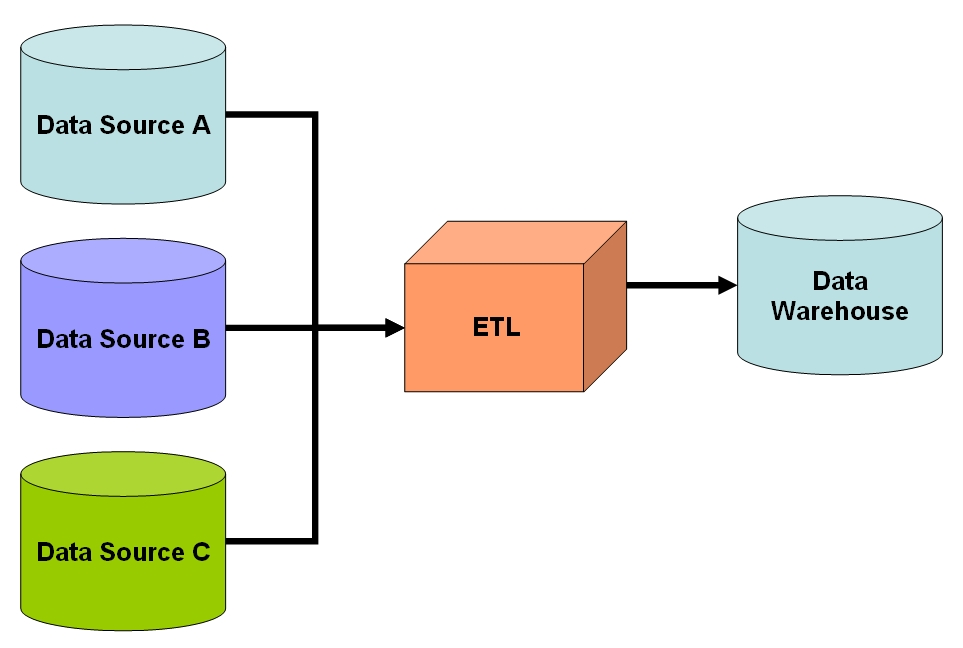
\includegraphics[width=280pt]{ETL+Datawarehouse.jpg}
    \caption{Sistema di Data Integration basato sull'approccio ETL con memorizzazione in Data Warehouse (Immagine tratta da da Wikipedia\cite{Integration-Wiki})}
    \label{fig:ETL_Datawarehouse}
\end{figure}

\vspace{5mm} %5mm vertical space

L'approccio ETL è composto, come dice il nome, da tre fasi distinte:
\begin{itemize}
\item estrazione, consiste nel ricavare dalle varie fonti (file, database, etc..) i dati utili al processo, nel nostro caso si tratta delle informazioni estratte in precedenza dai file CSV e DXF;
\item trasformazione, cioè l'applicazione di tutte le trasformazioni utili ai dati affinché possano essere utilizzati dall'utente finale, per il processo da noi sviluppato si tratta di applicare le procedure descritte in precedenza (Data Filtering e Data Validation) e di definire una nuova procedura per l'unificazione dei dati;
\item caricamento, si intende la memorizzazione dei dati provenienti dalla fase di trasformazione in un database definibile per la maggior parte dei casi come un Data Warehouse.
\end{itemize}

\newpage

Con il termine Data Warehouse si vuole definire un archivio di dati informatico (database) il quale memorizza le informazioni inerenti a un'azienda o ad un'organizzazione.
L'approccio del Data Integration basato su ETL e Data Warehouse pur essendo molto intuitivo e di vecchia concezione risulta tutt'oggi adatto ad essere implementato in sistemi che non richiedono un aggiornamento frequente dei dati.

\vspace{5mm} %5mm vertical space

Negli ultimi anni la tendenza per quanto riguarda i meccanismi di Data Integration è cambiata: grazie alle nuove tecnologie gli accessi a database, anche remoti, risultano molto più veloci e le applicazioni moderne si basano per lo più su dati in continua evoluzione e sempre aggiornati.
Ciò viene definito architettura con schema globale ed ha portato ad un minor impiego della logica ETL e ad un maggior utilizzo di interrogazioni (query) combinate su più database.
In questo modo si viene e creare un database virtuale i cui dati sono gli stessi dei database reali: tali informazioni vengono reperite ed elaborate in tempo reale tramite wrapper (involucri).

\begin{figure}[H]
    \centering
    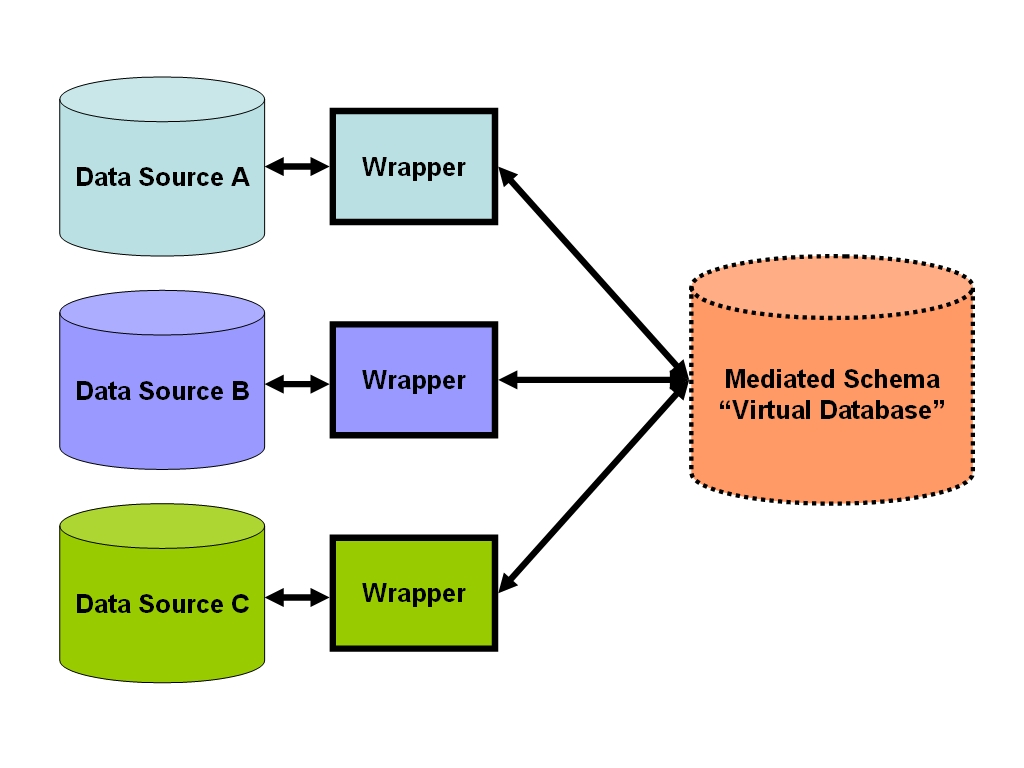
\includegraphics[width=280pt]{Dataintegration+Wrapper.jpg}
    \caption{Architettura con schema globale: Data Integration basato su un approccio di Database virtuale e wrapper (Immagine tratta da Wikipedia\cite{Integration-Wiki})}
    \label{fig:Data_Integration_Wrapper}
\end{figure}

\newpage

Il ruolo del wrapper in questo tipo di sistemi è riconducibile all'Adapter Pattern: il suo scopo è quello di rendere possibile la comunicazione tra due componenti le cui interfacce non corrispondono.

\begin{figure}[H]
    \centering
    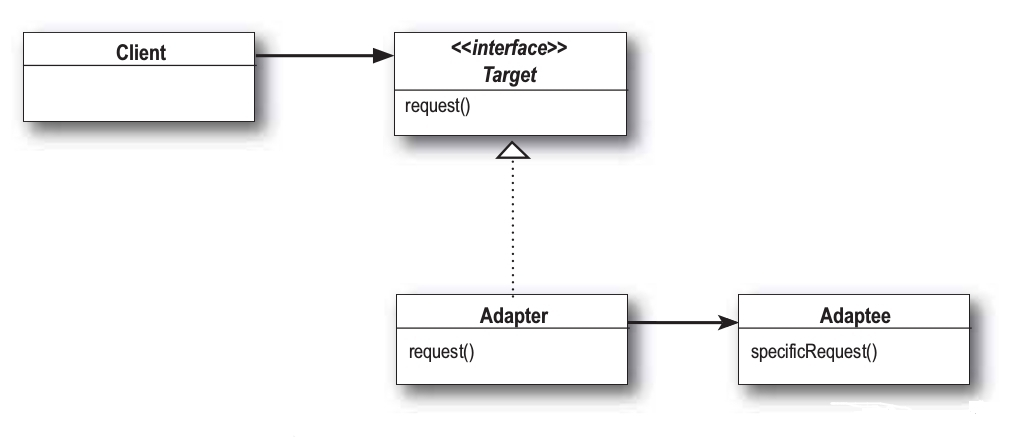
\includegraphics[width=280pt]{Adapter.jpg}
    \caption{Class Diagram UML dell'Adapter Pattern (Immagine tratta da \textit{Head First Design Patterns}\cite{Pattern})}
    \label{fig:Adapter_Pattern}
\end{figure}

\vspace{5mm} %5mm vertical space

L'architettura con schema globale può essere definita in due modalità base:
\begin{itemize}
\item GAV (Global As View), in cui lo schema globale viene espresso in base agli schemi delle sorgenti;
\item LAV (Local As View), dove lo schema globale è indipendente dalle sorgenti e la relazione con ognuna di esse è definita tramite delle view\footnote{Una view o vista consiste nel risultato di una query utilizzabile come se fosse una tabella.}. 
\end{itemize}

L'approccio GAV è di più immediata realizzazione ma in caso di cambiamenti nelle fonti, come l'aggiunta di una nuova sorgente, risultano complesse le modifiche da apportare.
Viceversa il LAV favorisce le possibili estensioni rispetto a nuove sorgenti ma risulta più complicato definire le query utili alla sua definizione.     

Per GLAV (Global and Local As View) si intende un ibrido tra le due strategie appena descritte: in questo caso la relazione tra le sorgenti e lo schema globale è stabilita attraverso delle view, alcune definite sullo schema globale e alcune sulle sorgenti.

\vspace{5mm} %5mm vertical space

Dato che il progetto Spazi-Unimi prevede di operare principalmente su dati edilizi i quali risultano statici a meno di rare variazioni (ad esempio un cambio di sede per un dipartimento, ristrutturazioni, cambi di destinazione delle stanze) si è deciso di implementare un sistema ETL che definisce un database di tipo Data Warehouse.


\newpage
\section{Analisi dei dati (da DXF e CSV)}

Volendo applicare l'approccio ETL del Data Integration e avendo già effettuato l'estrazione dei dati dai file forniti ci si è concentrati sulla fase di trasformazione nella quale bisogna innanzitutto applicare il Data Filtering e il Data Validation.
Per utilizzarli in maniera efficace la prima operazione da fare è un'analisi approfondita delle informazioni provenienti dalle varie fonti in modo da capire i livelli di accuratezza, completezza e consistenza dei dati.

\vspace{5mm} %5mm vertical space

L'analisi è stata effettuata innanzitutto sui tre file CSV forniti dalla Divisione Manutenzione edilizia e impiantistica; i fogli elettronici contenevano informazioni su: edifici, aule ed infine categorie delle stanze.
Il file degli edifici contiene i seguenti dati per ogni palazzo rappresentato:
\begin{itemize}
\item legacy\_building\_id\footnote{Con il termine legacy si vuole indicare una caratteristica ereditata da un vecchio sistema la quale viene ancora utilizzata in certi casi particolari.}, cioè l'identificatore del vecchio standard per il palazzo, è presente per ogni edificio;
\item building\_id, il nuovo identificatore di palazzo, è presente solo per gli edifici che hanno messo in pratica il nuovo standard di identificazione cioè l'83,7\% (206 su 246);
\item address, l'indirizzo è sempre presente per ogni edificio ma non viene utilizzato sempre lo stesso standard di codifica e in molti casi il contenuto risulta poco utile (ad esempio: `LODI OSPEDALE VETERINATRIO Ed. 1');
\item lat e lon, le coordinate dell'edificio non indicano sempre lo stesso punto per ogni edificio (ad esempio l'ingresso), inoltre non sono presenti in 51 edifici cioè nel 20,7\% dei casi.
\end{itemize}

\vspace{5mm} %5mm vertical space

Il file CSV con le informazioni sulle aule didattiche della Divisione edilizia contiene: %PROF: come mai qui hai usato una "barreviazione" del nome della divisione? Uniformare... controlla anche il resto del documento
\begin{itemize}
\item building\_id, corrispondente a uno di quelli del file degli edifici, tale dato è sempre presente per ogni aula e risulta utilissimo per definire in che palazzo si trova tale stanza;
\item address, informazione ridondante rispetto al file precedente, è sempre presente per ogni aula;
\item legacy\_floor, identificativo proprio della divisione edilizia per indicare in che piano si trova l'aula, l'informazione è sempre presente ma non è di immediata lettura e il livello di accuratezza si può verificare solo controllando stanza per stanza sulle piantine fornite;
\item room\_id, identificativo dell'aula risulta univoco solo all'interno di uno stesso palazzo, è sempre presente e combinandolo con il building\_id può fornire una chiave univoca per l'identificazione della stanza;
\item cat\_name, definisce la destinazione d'uso della stanza, è sempre presente anche se in questo file sono contenuti solo i dati delle aule didattiche (aule, aule informatiche, sale lauree, etc.);
\item room\_name, indica il nome con cui viene chiamata la stanza, è molto utile dal lato utente dato che verrà sicuramente usato per la ricerca di aule di interesse, il dato è presente nel 90,8\% dei casi (367 aule);
\item capacity, indica la capienza dell'aula ed è presente nel 93\% dei casi (376 aule su 404);
\item area, indica la superficie della stanza in metri quadrati, non risulta molto utile agli scopi dell'applicazione nonostante il dato sia presente in quasi tutte le stanze rappresentate;
\item buiding\_name, indica una denominazione specifica dell'edificio a cui la stanza appartiene, l'informazione risulta poco utile dal lato utente perché spesso contiene nomi utili alla divisione edilizia, il dato è comunque presente nella maggior parte dei casi;
\item note, informazioni aggiuntive sull'aula, poco presenti e di interesse nullo per gli scopi dell'applicazione.    
\end{itemize}

\vspace{5mm} %5mm vertical space

L'ultimo file fornito dalla Divisione Manutenzione edilizia e impiantistica è quello sulle categorie delle stanze:
\begin{itemize}
\item category\_id, identificatore della categoria utilizzato nelle etichette delle stanze nei file DXF, risulta utilissimo per capire di che tipologia di stanza si sta parlando; è sempre presente per ogni categoria;
\item category\_name, è il nome `umano'  della categoria di stanza; è sempre presente e fornisce all'utente una denominazione comprensibile delle tipologie di aule.
\end{itemize} 

\newpage

La fase successiva è stata l'analisi dei CSV forniti dalla Divisione sistemi informativi (EasyRoom) iniziando sempre da quello degli edifici:
\begin{itemize}
\item building\_id, l'identificativo del palazzo in questo caso utilizza sempre la nuova codifica ed è sempre presente anche se 8 edifici su 51 possiedono un identificativo provvisorio dato che non contengono ancora dati precisi;
\item building\_name, il nome dell'edificio è sempre presente ma è in molti casi troppo generico rispetto alle informazioni fornite dalla Divisione edilizia;
\item address, l'indirizzo manca nel 7,8\% (4 edifici su 51) dei casi ma risulta ben formato rispetto a quelli forniti dal CSV corrispettivo dell'edilizia;
\item n\_floor, indica il numero di piani dell'edificio, l'informazione risulta %PROF: intendi per noi? perché easyroo non ha i file DXF, quindi per loro non è ridondante
ridondante dato che è riconducibile al numero di file DXF forniti per quel palazzo inoltre è poco verificabile ma risulta sempre presente;
\item google\_maps\_address, indica un iframe\footnote{Un iframe è un elemento HTML utilizzato solitamente per mostrare il contenuto di una pagina web.} contenente l'indirizzo web della pagina di Google Maps corrispondente al palazzo, da esso si potrebbero ricavare le coordinate ma nonostante siano quasi sempre presenti risulta molto più comodo %PROF: comodo? riguardo all'affidabilità sono paragonabili?
ottenerle dal CSV dell'edilizia. 
\end{itemize} 

\vspace{5mm} %5mm vertical space

L'ultimo file CSV da analizzare è stato quello dei sistemi informativi contenente le informazioni sulle aule didattiche da loro conosciute:
\begin{itemize}
\item room\_id in questo caso contiene l'identificatore dell'edificio separato con un `\#' dall'identificatore della stanza; il dato è sempre presente anche se in alcuni casi risulta non rispettato lo standard appena descritto e viene utilizzato un nome per definire l'aula;
\item room\_name è il nome umano della stanza; è sempre presente e come per il file CSV corrispettivo risulta molto utile per la ricerca di aule degli utenti;
\item building\_id, informazione ridondante dato che è contenuta anche dal room\_id, è sempre presente ma come per il file di edifici utilizza anche identificatori provvisori non utilizzabili dall'applicazione;
\item venue, indica la sede contenente l'aula; è sempre presente ma come in precedenza utilizza nominativi troppo generici rispetto alle informazione dell'edilizia;
\item capacity indica la capienza dell'aula; è sempre presente anche se le informazioni fornite dall'edilizia possono sembrare in tale ambito più affidabili;
\item type indica la tipologia di grandezza dell'aula classificandola in `Piccola', `Media' o `Grande'; l'informazione è sempre presente ma risulta troppo generica e poco utile all'utente finale;
\item available indica la possibilità di utilizzarla previa richiesta; il dato è sempre presente ma indica un risposta negativa per ogni aula quindi non risulta utilizzabile;
\item equipments elenca gli accessori presenti in tale aula (proiettore, pc, lavagna luminosa, etc.); il dato è presente in molte aule e se non presente si può presupporre che la stanza non abbia nessun accessorio;
\item description, descrizione della destinazione d'uso della stanza, risulta presente in circa la metà dei casi ma è troppo generica (ad esempio: `tradizionale') e non corrisponde quasi mai allo standard utilizzato dall'edilizia;
\item legacy\_floor, piano in cui si trova l'aula, utilizza uno standard basato sui numeri interi quindi risulta più comprensibile rispetto al dato fornito dall'edilizia; l'informazione non è presente solo per 2 stanze ma risulta difficile dedurne l'affidabilità;
\item accessibility indica la possibilità da parte di una persona disabile di accedere alla stanza; è rappresentata con un numero (`0' se non è possibile, `1' se lo è) ed è sempre presente nelle stanze conosciute dalla Divisione sistemi informativi. Il dato inoltre è molto utile ai fini degli utenti finali dell'applicazione. 
\end{itemize}

\vspace{5mm} %5mm vertical space

L'ultima attività di analisi dei dati per il progetto ha riguardato le piantine contenute nei file DXF nei quali le informazioni più importanti oltre a quelle di disegno sono:
\begin{itemize}
\item il nome del file nel cui prefisso è indicato il legacy\_building\_id dell'edificio cioè il codice nel vecchio standard;
\item il piano rappresentato dalla piantina del quale ci si è occupati nella lettura del file;
\item le etichette contenute nei layer `NLOCALI' e `RM\$TXT' riguardanti le aule.
\end{itemize}  

\newpage

Nelle etichette di ogni aula sono stati identificati i seguenti dati:
\begin{itemize}
\item il room\_id della stanza contenuto in entrambi i layer testuali;
\item il category\_id della stanza mappabile nel nome della categoria grazie al CSV corrispondente della Divisione Manutenzione edilizia e impiantistica;
\item la metratura della stanza quasi sempre presente ma di scarso valore per gli scopi dell'applicazione.
\end{itemize}  

\vspace{5mm} %5mm vertical space

Terminata l'analisi di tutti i dati provenienti dalle varie fonti è stato definito per ogni file CSV l'insieme delle informazioni ritenute utili al progetto: ogni dato non presente in tale insieme è stato quindi scartato.

Dopo aver inferito la tipologia del file CSV viene quindi applicato un filtro che mantiene solo le colonne ritenute importanti. 
La scrematura si basa ancora una volta sui dizionari degli header salvati in `general.json': è bastato perciò applicare al dizionario ottenuto dalla lettura del CSV una funzione che filtra le chiavi.
\begin{python}[title=Definizione della funzione filter\_keys, frame=single]
def filter_keys(d, valid_keys):
   return { k: d[k] for k in d if k in valid_keys }
\end{python}

\vspace{5mm} %5mm vertical space

Il file CSV contenente le categorie delle stanze fornito dall'edilizia presenta dei dati totalmente statici il cui aggiornamento porterebbe ad una revisione totale dei file DXF.
Tale cambiamento risulta di estrema difficoltà. Per tale motivo e anche per la necessità di operare su tali categorie in maniera da poterle rendere più utilizzabili per gli utenti si è deciso di togliere la possibilità di aggiornare tali informazioni tramite CSV.
Utilizzando un file JSON infatti si è riusciti ad avere le stesse informazioni del CSV estese così da poter raggruppare le categorie per similarità di tipologia e di scopo. 
Il risultato finale è stato un dizionario avente come chiavi i category\_id e come valori il nome del gruppo di appartenenza (group\_name), la descrizione (category\_name tratta dal file CSV) e lo scopo generico (scope) a cui la stanza è destinata.

\newpage

\begin{dict}[title=Esempio delle categorie di stanze memorizzate in `room\_categories.json', frame=single]
"AUM01" : {
   "group_name"   : "Aula Seminari - Magna - Lauree",
   "description"  : "Aula Magna",
   "scope"        : "didactic"
},

"LAB01" : {
   "group_name"   : "",
   "description"  : "Laboratorio Didattico",
   "scope"        : "didactic"
},

"SAL04" : {
   "group_name"   : "Aula Seminari - Magna - Lauree",
   "description"  : "Sala Lauree",
   "scope"        : "didactic"
},

"SPZ01" : {
   "group_name"   : "Locale Supporto",
   "description"  : "Locale di Supporto",
   "scope"        : "support"
}
\end{dict}

\vspace{5mm} %5mm vertical space

In alcuni casi la tipologia di aula data la sua rilevanza non ha permesso il raggruppamento con altre: in questo caso il group\_name è stato lasciato vuoto.

Per poter utilizzare correttamente i dati contenuti in tale file JSON è stata implementata la classe RoomCategory che definisce i metodi utili ad ottenere le informazioni sulle categorie partendo da un category\_id o da una description.


\newpage
\section{Salvataggio dei dati in MongoDB}

La fase successiva del processo di Data Integration applicato prevederebbe il merge dei dati in modo da poterli caricare sul database e renderli disponibili all'applicazione finale.
Nel nostro caso però si è deciso di passare per uno step intermedio che prevede la memorizzazione dei dati di ogni edificio in un unico documento separandoli su chiavi diverse in base alla fonte di provenienza.
Questa scelta è stata fatta in funzione di due fatti:
\begin{itemize}
\item MongoDB essendo un database NoSQL prevede un costo in termini di spazio di memorizzazione minore rispetto ai DB classici quindi la ridondanza delle informazioni è un fattore positivo perché spesso evita query complesse;
\item per effettuare l'unione delle informazioni di un palazzo bisogna attendere che i dati di tutte le fonti siano presenti: ciò nel nostro caso può richiedere molto tempo (se ad esempio una fonte non aggiorna in maniera puntuale i propri file) quindi risulta utile memorizzare i dati separati per poi applicare su di essi il processo di merge. %PROF: forse spiegabile meglio parlando direttamente di differenza di frequenza di aggiornamenti dei file    
\end{itemize}

\vspace{5mm} %5mm vertical space

Una volta definite le classi con lo scopo di leggere i dati dalle due tipologie di file a disposizione quindi si è deciso di implementare un programma principale ('main') dal quale richiamare con gli appositi comandi il processamento dei file.
I comandi implementati sono stati:
\begin{itemize}
\item dxf file.dxf, al comando `dxf' si passa uno o più file DXF da processare;
\item csv file.csv, il comando `csv' come l'altro può ricevere uno o più file di tipologia corretta. 
\end{itemize}

Tali comandi dopo avere controllato l'estensione e la presenza dei file indicati istanziano un apposito `task': il compito di tali classi (DXFTask e CSVTask) è quello di richiamare tutte le operazioni da effettuare sui file.
La prima operazione da effettuare è la lettura e per fare ciò viene richiamata la classe corrispondente (DXFReader o CSVReader). 
I risultati della lettura vengono quindi passati alle corrispondenti classi che hanno il compito di aggiornare i dati presenti nel database (o, se è il caso, di inserirli per la prima volta). 

\vspace{5mm} %5mm vertical space

Le classi definite per effettuare queste operazioni sono: DXFDataUpdater, EdiliziaDataUpdater e EasyroomDataUpdater. 
La prima si occupa, come indica il nome, di ricevere i risultati del DXFReader, cercare il palazzo corrispondente nel database e salvare tali dati nella chiave `dxf' del documento. 
Nel caso in cui l'edificio non sia presente nel database viene creato un nuovo documento e salvato nella collection `building'; se invece il documento è già presente e possiede una chiave `dxf' con il piano corrispondente esso viene sostituito dai nuovi dati letti.
Dato che DXFReader ritorna un oggetto di tipo Floor i dati che vengono salvati sono quelli del JSON ottenuto dal suo metodo \textit{to\_serializable()} che ritorna un dizionario. 

Il CSVReader come detto riesce grazie agli header ad inferire la tipologia del file (sorgente e tipo di dati), grazie a ciò il CSVTask istanzia una classe di aggiornamento specifica rispetto alla fonte corrispondente.
EdiliziaDataUpdater si occupa di aggiornare i dati provenienti dai CSV della Divisione Manutenzione edilizia e impiantistica; EasyroomDataUpdater invece si occupa di quelli della Divisione sistemi informativi.
Entrambi i Data Updater si devono occupare di due possibili input: le informazioni sulle stanze o le informazioni sugli edifici.
Essendo le operazioni da svolgere su tali informazioni molto simili si è deciso di definire altre due classi che implementassero le funzionalità comuni e da cui i Data Updater ereditassero:
\begin{itemize}
\item BuildingDataUpdater si occupa delle operazioni comuni ai dati sugli edifici come trovare i documenti da aggiornare e controllare la validità di dati quali il building\_id;
\item RoomDataUpdater invece oltre a trovare l'edificio in cui salvare i dati e validare il room\_id raggruppa le stanze di uno stesso palazzo in piani, in questo modo sul database avremo per ogni edificio una lista di piani ordinata in cui sono contenute le informazioni delle stanze.
\end{itemize}
Altri tipi di operazioni da svolgere prima del salvataggio invece sono diverse in base alla fonte da cui provengono i dati: per questo motivo EasyroomDataUpdater ed EdiliziaDataUpdater sono state mantenute come due classi separate.

Un esempio è dato dal room\_id proveniente dalla Divisione sistemi informativi: come detto esso è composto dall'identificatore della stanza e da quello dell'edificio (separati da un `\#'). Avendo già l'informazione sul building\_id presente in un altro campo si è deciso di modificarlo prima del salvataggio filtrandolo così da lasciare solo il room\_id.

Un'altra operazione sui dati che va effettuata solo per una delle due fonti è la validazione dell'indirizzo dei palazzi conosciuti dalla Divisione Manutenzione edilizia e impiantistica.
Tali indirizzi seguono spesso uno standard preciso: città, via, numero civico e se presente il numero di edificio rispetto al complesso in cui si trovano. 
Altre volte come detto nell'analisi dei dati l'indirizzo non fornisce delle informazioni esatte sulla posizione del palazzo.
Si è quindi deciso nella procedura \textit{sanitize\_building} di analizzare tale valore di indirizzo in modo da uniformarlo quando lo si ritiene utile mentre in caso contrario viene segnalato il problema e il campo viene lasciato vuoto.
Nel caso in cui si riesca anche ad estrarre il numero di edificio questo viene memorizzato in attributo specifico.
 
\vspace{5mm} %5mm vertical space

La politica che si è voluto implementare per quanto riguarda gli aggiornamenti è detta a `snapshot'\footnote{Il termine snapshot significa letteralmente istantanea.}: lo stato del database rispecchia quello delle informazioni possedute in quel momento senza andare a memorizzare vecchi dati.
Questo approccio è stato mantenuto sia per i dati provenienti dai file CSV che dai DXF: ogni chiave ('dxf', `edilizia', `easyroom') del documento possiede un valore updated\_at contenente la data precisa di aggiornamento, tale attributo è presente anche per il documento stesso e corrisponde al più recente delle tre possibili chiavi.

Il caso più critico in tale approccio si ha quando un edificio non deve più essere contenuto nel database perché ad esempio non viene più utilizzato dall'università.
In tale situazione si può fare una semplice assunzione: essendo i file CSV globali essi contengono i dati di ogni edificio perciò se un edificio presente in uno stato precedente non si trova in un nuovo aggiornamento allora è da considerarsi eliminato.
Controllando l'attributo updated\_at si riesce a capire quali edifici non sono descritti in un file CSV quindi si può procedere alla rimozione della chiave corrispondente alla fonte aggiornata.
In un attributo dell'edificio (deleted\_keys) inoltre si provvede a specificare quali chiavi sono state eliminate: in questo modo se `easyroom' ed `edilizia' sono sono state rimosse significa che entrambe le fonti concordano sulla cancellazione dei dati e il documento di tale edificio può essere rimosso.

Tutte le operazioni di controllo sugli aggiornamenti e sulla cancellazione di chiavi e documenti sono effettuate dal BuildingDataUpadater.
La chiave `dxf' non viene presa in considerazione per quanto riguarda la cancellazione di un edificio dal database in quanto i file si occupano solo di un piano per volta quindi risulterebbe difficile definire una strategia di cancellazione basata sul loro aggiornamento.    

\vspace{5mm} %5mm vertical space

Per operare in maniera efficiente sul database si è deciso di implementare alcune classi di supporto in modo da rendere le operazioni più semplici.
La classe DB è molto semplice e si occupa esclusivamente della connessione al database dell'applicazione; per fare ciò utilizza la libreria esplorata all'inizio del processo: Pymongo.

MongoDBPersistenceManager invece importa DB per la connessione ed il suo compito è quello di definire dei metodi per effettuare le operazioni sul database.
Tali metodi sono già realizzati da Pymongo e quindi non si necessiterebbe di un ulteriore livello come quello fornito da tale classe.
L'idea di base però è quella di rendere il sistema disaccoppiato dalle logiche del database così che un possibile cambio nella sua tipologia risulterebbe molto più semplice.

ODMModel (che eredita da ODMAttrs) è invece una classe con lo scopo di definire un ODM (Object Document Mapping) per il caso specifico di MongoDB.
Un ODM ha l'obbiettivo di fornire i servizi di persistenza sui dati di un database utilizzando un'interfaccia orientata ai documenti.
Nonostante la presenza di ODM già disponibili per Python si è deciso di definire da zero questa classe in quanto le implementazioni già esistenti sono risultate dei veri e propri framework per la manipolazione del database.
In paragone a tali librerie ODMModel è risultata molto più leggera dato che implementa solo le funzionalità a noi utili.

Grazie ai metodi ridefiniti in MongoDBPersistenceManager e all'ODMModel si riesce quindi ad ottenere una mappatura intuitiva tra i documenti del database e gli oggetti di Python.

Per poter salvare i dati nella collection `building' in maniera semplice è quindi stata definita la classe Building che ereditando da ODMModel può utilizzare tutti i metodi per operare sul database in maniera ottimale.


\newpage
\section{Merge dei dati}

Le operazioni di unione dei dati dette più comunemente merge sono la parte fondamentale della fase di trasformazione delle informazioni per quanto riguarda il nostro approccio di Data Integration.
Come detto i dati provenienti dalle varie fonti sono stati già elaborati e posti in chiavi separate degli stessi documenti ognuno dei quali rappresenta un edificio.
Vi sono però alcune operazioni preliminari, riconducibili al concetto di merge, che per comodità sono state inserite nelle fasi precedenti di elaborazione cioè nei Data Updater.

Innanzitutto i documenti salvati nel database utilizzano come identificativo il building\_id quindi il nuovo standard; in caso la sorgente non utilizzasse tale standard viene utilizzato il legacy\_building\_id cioè il vecchio standard degli identificativi.
In questo modo però si vengono a salvare documenti separati per informazioni riguardanti lo stesso palazzo; ad esempio i dati tradotti dai file DXF avrebbero come identificativo il `legacy' mentre quelli provenienti dalla Divisione sistemi informativi utilizzerebbero il nuovo standard.
La soluzione sta nel file CSV fornito dall'edilizia che contiene i dati sugli edifici: esso è l'unico contenente una mappatura tra i due diversi standard.
Tale mappatura è utilizzata nella fase di salvataggio in due modi:
\begin{itemize}
\item nel caso in cui la fonte utilizzi il vecchio standard si cercano i documenti non in base all'identificatore ma in base all'attributo `l\_b\_id' (legacy\_building\_id);
\item all'inserimento del file sugli edifici dell'edilizia si richiama una procedura che cerca i documenti che usano come identificatore il vecchio standard e li modifica in modo che utilizzino il nuovo `id' reso ora disponibile dal CSV. 
\end{itemize} 

\vspace{5mm} %5mm vertical space

Le altre due operazioni di unificazione dei dati da applicare in lettura dei file riguardano i dati delle piantine: l'identificazione della categoria delle stanze e l'identificazione delle stanze di cui si hanno informazioni provenienti dalle altre fonti.

Come detto in precedenza le etichette lette nei file DXF vengono associate ad una stanza in base alla loro posizione e salvate come testi; entrambe le operazioni da effettuare quindi devono solamente ciclare sulle stanze e poi sui loro testi per confrontarli con gli identificativi di categoria o di stanza.

L'identificazione della categoria comporta per la procedura corrispondente la creazione per tale stanza di un attributo `cat\_id' col quale è quindi possibile accedere in maniera posizionale alla voce corrispondente del dizionario in `room\_categories.json'. 
Il testo attraverso il quale è stata inferita la tipologia di stanza viene quindi rimosso dalla lista dato che ha terminato il suo compito e non ha più utilità per il sistema.

L'identificazione della stanza invece prevede che siano già stati inseriti i file CSV contenenti le informazioni sulle aule; con tali informazioni si possono confrontare i room\_id con i testi delle etichette e cercare delle corrispondenze.
Trovata una stanza che matcha con un identificatore la si sposta dalla lista di stanze trovate nel DXF (chiamata unmatched\_rooms) e la si pone in un nuovo attributo strutturato come un dizionario in cui si utilizza proprio il room\_id come chiave. 

\vspace{5mm} %5mm vertical space

Il merge delle informazioni di un documento prevede di utilizzare i dati presenti nelle chiavi separate (`dxf', `edilizia', `easyroom') per definire il contenuto di una nuova chiave denominata `merged'.
Le operazioni di merge sono divisibili in due fasi principali: l'unione delle informazioni sugli edifici e l'unione di quelle sulle stanze.

La prima fase essendo la più facile da implementare è anche stata la prima; le informazioni sugli edifici infatti provengono solo dai due file CSV (dell'edilizia e dei sistemi informativi).
La classe che si occupa del lavoro di merge sui dati è il "DataMerger" e implementa il metodo \textit{merge\_builging} che riceve le informazioni delle chiavi `edilizia' ed `easyroom'. Tale metodo si occupa poi di richiamare dei metodi ausiliari che provvedono a ritornare campo per campo l'informazione migliore da salvare. I dati ricavati e salvati da merge\_building sono:
\begin{itemize}
\item legacy\_building\_id, tale dato come noto è conosciuto solo dalle informazioni provenienti dall'edilizia quindi \textit{\_merge\_building\_l\_b\_id} ritorna tale identificatore se è presente altrimenti una stringa vuota;
\item address, l'indirizzo dell'edificio come visto in analisi dei dati è migliore se preso dalla Divisione sistemi informativi, se non è presente si utilizza quello validato proveniente dall'edilizia e se nessuno dei due esiste si ritorna una stringa vuota;
\item building\_number, tale informazione è ricavata solo dalla validazione dell'indirizzo dell'edilizia, se non c'è viene ritornato `None'\footnote{Il valore None in Python è l'equivalente del Null in Java cioè il valore nullo.};
\item building\_name, questa volta l'informazione proviene solo da easyroom e se non esiste \textit{\_merge\_building\_name} ritorna una stringa vuota;
\item coordinates, le coordinate se presenti nella chiave `edilizia' vengono validate ed utilizzate, se mancano viene utilizzato l'indirizzo di easyroom per ricavarle facendo richiesta ad un'apposita libreria di geocoding\footnote{\url{https://pypi.python.org/pypi/pygeocoder}}. 
\end{itemize}

\vspace{5mm} %5mm vertical space

Le coordinate prima di essere salvate nella chiave `merge' devono essere passate al metodo \textit{\_prepare\_GeoJson\_coordinates} che le trasforma nel formato GeoJson utilizzato da MongoDB proprio per la loro memorizzazione.

Tutti gli attributi ottenuti mergiando le informazioni delle fonti usate vengono validati prima di essere salvati: se un attributo risulta vuoto (o nullo) viene rimosso così da non avere valori nulli nella chiave `merge'.

\vspace{5mm} %5mm vertical space

La procedura di unificazione dei dati sulle aule invece è risultata molto più complessa da implementare in quanto tali dati provengono da tre fonti diverse (i file DXF e i due file CSV sulle aule) le quali non sempre risultano corrette per quanto riguarda alcune informazioni. Il fatto di aver salvato le aule in piani separati contenuti in una lista ha inoltre complicato la progettazione.

La funzione \textit{merge\_floors} si occupa di ritornare la lista ordinata di piani contenenti i dati mergiati; tale funzione deve utilizzare tre sorgenti che però non sono sempre presenti nel database: per questo motivo tutte le operazioni sui dati lavorano solo su due fonti per volta.
In questo modo alla prima iterazione le prime due fonti verranno unite e il risultato parziale verrà poi unito alla terza fonte.

La criticità nel merge delle informazioni riguardanti le aule è stata riscontrata nel fatto che in alcuni casi l'indicazione del piano di una fonte varia rispetto alle altre: in questo modo risulta difficile capire dove si trova realmente una stanza senza andare a controllare sul posto.
La soluzione è stata trovata ragionando su quale fonte sembrasse maggiormente affidabile: il risultato di questa domanda è stato l'ordinare le chiavi in base alla loro attendibilità.
La fonte con affidabilità maggiore per quanto riguarda il raggruppamento delle aule in piani è risultata senza ombra di dubbio quella dei DXF: se una stanza si trova nello stesso piano delle altre sicuramente sarà disegnata nella stessa piantina. L'ordinamento delle due fonti CSV invece è il risultato di un'esplorazione più approfondita dei casi critici riscontrati: il CSV proveniente dalla Divisione Manutenzione edilizia e impiantistica contenendo meno errori di quello della Divisione sistemi informativi ha ricevuto una maggiore priorità.

La maggior affidabilità della fonte ha portato all'esecuzione in maniera prioritaria delle sue informazioni nella procedura di merge dei floor: la fonte presente con maggior attendibilità viene utilizzata come base per le operazioni di unificazione dei dati.
`edilizia' (la seconda per priorità). Il risultato di tale merge viene poi passato alla stessa procedura con la chiave rimanente cioè `easyroom'.

La funzione \textit{match\_and\_merge\_floors} riceve una lista di piani dalla sorgente `base' e si occupa di ciclare piano per piano associando le stanze provenienti dall'altra fonte. I piani vengono trattati come nella teoria degli insiemi quindi dall'insieme totale delle aule della sorgente secondaria viene tolta l'intersezione con l'insieme del piano base su cui si sta operando. In questo modo alla fine del ciclo sui piani base si potrebbero avere delle aule non risultanti in nessun piano: in questo caso si controlla dove è andato a finire l'insieme con cardinalità maggiore delle aule aventi lo stesso identificativo di piano e si associa la stanza allo stesso.

A questo punto si passano alla funzione \textit{\_merge\_rooms\_into\_floor} i seguenti parametri per ogni piano: un piano proveniente dalla fonte prioritaria, un piano proveniente dalla fonte con minor priorità e un set di room\_id.
Per ogni stanza indicata nel set la procedura si occupa di trovare le informazioni ottenibili dalle due sorgenti in modo da richiamare la funzione \textit{merge\_room} la quale ritorna le informazioni unificate dell'aula.

La funzione \textit{merge\_room} riceve quindi le informazioni di due fonti diverse senza però sapere quali esse siano vista la natura dell'algoritmo implementato.
I dati presenti sulle aule però risultano provenienti quasi sempre da sorgenti diverse quindi l'unica cosa che tale procedura fa è quella di controllare se le informazioni sono presenti ed utilizzare quelle della prima fonte disponibile.
Unica eccezione a questo modo di operare è data dall'attributo che indica la categoria della stanza: essendo nei DXF tale informazione dipendente dalla posizione delle etichette si è preferito utilizzare sempre le fonti con minor priorità (che saranno `edilizia' o `easyroom') ritenute in questo caso più affidabili.
La motivazione sta nell'aver riscontrato alcune criticità sul posizionamento di tali etichette soprattutto per quanto riguarda stanze molto piccole: in tali casi l'etichetta non essendo contenuta risulta associata a stanze vicine rischiando di provocare un errore nell'inferenza delle categorie.

\vspace{5mm} %5mm vertical space

Tutte le operazioni di merge sono quindi richiamabili tramite due singole funzioni: \textit{merge\_building} e \textit{merge\_floors}.
Tali procedure vanno quindi richiamate ogni volta che si deve rieseguire l'unione di dati a seguito di una modifica degli stessi.
Per evitare di creare un task specifico da richiamare manualmente da chi ha aggiornato i dati si è deciso di porre le chiamate dei metodi in punti chiave dell'aggiornamento dei dati.
\textit{merge\_building} viene richiamato nel BuildinDataUpdater quando vengono aggiornati i dati nelle varie chiavi, in questo momento le informazioni sono disponibili e una volta effettuato il merge ed aggiunta (o modificata) la chiave `merged' si può procedere ad un unico salvataggio nel database.
La procedura \textit{merge\_floors} invece può essere richiamata in tre punti diversi del codice:
\begin{itemize}
\item nel RoomDataUpdater cioè dopo l'aggiornamento dei CSV sulle aule;
\item nel DXFDataUpdater quindi in seguito all'aggiornamento di una piantina;
\item nell'EdiliziaDataUpdater in seguito all'unione di due documenti dovuta alla precedente memorizzazione con il legacy\_building\_id come identificatore.  
\end{itemize}    

Anche questa volta la procedura viene richiamata, il risultato posto nella chiave `merged' e il documento salvato nel database.

\vspace{5mm} %5mm vertical space

Giunti a questo punto ci si è resi conto della necessità di svolgere alcune operazioni sui dati esattamente prima del loro salvataggio nel database (o subito dopo).
Per richiamare queste operazioni si è quindi deciso di implementare in ODMModel una politica di `callback'. 

\newpage

Per callback si intende una funzione che viene passata come argomento ad un'altra con lo scopo di essere eseguita successivamente, ciò risulta molto utile quando per qualche ragione l'operazione non può essere subito effettuata.
Nel nostro caso sono state definite due tipologie di callback:
\begin{itemize}
\item sulla classe, eseguono il metodo sulla classe a cui è associato per ogni istanza esistente;
\item sulla istanza, eseguono il metodo una sola volta sulla istanza su cui viene richiamato. 
\end{itemize}

Come detto inoltre le callback possono venire richiamate sia prima del salvataggio (\textit{before\_callback}) sia dopo (\textit{after\_callback}).

La politica di callback viene utilizzata ad esempio per mantenere ordinate le liste di piani salvati nei documenti in MongoDB: la classe Building si occupa infatti di effettuare una callback passando la funzione \textit{ensure\_floors\_sorting}

\newpage
\section{Reporting degli errori e delle criticità}

Il progetto Spazi-Unimi oltre a voler realizzare uno strumento utile agli utenti dell'Università degli Studi di Milano ha un secondo scopo: fornire alle sorgenti dei dati un riscontro per quanto riguarda la loro qualità.
Dovendo gestire grosse moli di informazioni non è semplice trovare e correggere gli errori, ma grazie alle operazioni di Data Validation e Data Integration implementate si è riusciti a identificare errori e problemi ricorrenti.

Per fare in modo che gli addetti all'aggiornamento dei dati capiscano anche la qualità di quello che stanno inserendo nel sistema si è deciso di utilizzare una classe di log\footnote{Con il termine log in informatica si intende la registrazione delle operazioni svolte.} in modo da rendere l'output molto più leggibile per l'utente.

La classe Logger può essere richiamata grazie ad alcuni tipi di funzioni in base al contesto in cui ci si trova:
\begin{itemize}
\item info, l'etichetta è di colore blu ed indica cosa sta elaborando in quel momento il sistema o mostra alcuni dati parziali;
\item warning, l'etichetta arancio viene mostrata in caso di criticità nell'esecuzione di qualche algoritmo, il problema non pregiudica però l'esecuzione;
\item error, l'etichetta è rossa ed indica un errore grave che il sistema non è in grado di risolvere, l'esecuzione di tale operazione è interrotta e si passa all'iterazione successiva;
\item success, l'etichetta verde indica la conclusione del programma mostrando le statistiche sui tempi di esecuzione.
\end{itemize}    

\vspace{5mm} %5mm vertical space

Grazie all'uso dell'indentazione si è cercato di rendere l'output più semplice da capire; inoltre l'utente che aggiorna i dati può settare tramite una variabile il livello di verbosità del Logger così da visualizzare solo le informazioni di suo interesse (ad esempio si possono visualizzare solo gli `error' e le `info' associate).

Le chiamate alla classe Logger quindi sono utilizzate in maniera esaustiva in tutte le procedure svolte dal sistema in modo da semplificare il compito degli addetti.

\newpage

%PROF: nell'oytput seguente la scritta in warn in giallo è illeggibile causa colore... mettere un arancione?
\begin{outputl}[title=Esempio di output del Logger nel processamento di file DXF, frame=single]
[info] 0/3 - Processing file assets/dxf/Con audit/5830_1.dxf
       [warn] Self crossing room is not valid: 
       Polygon(P(8566.2958, -7802.069))[P(0.0, 125.0), 
       	P(312.0, 125.0), P(312.0, 315.0), P(136.0, 315.0), 
       	P(136.0, 332.0), P(441.0, 332.0), P(441.0, 104.0), 
       	P(312.0, 104.0), P(312.0, 125.0), P(0.0, 125.0), 
       	P(0.0, 0.0), P(531.4215, 0.0), P(541.6033, 308.0), 
       	P(0.0, 0.0), P(0.0, 125.0)]
       [info] Floor 10 for Building Id: 33110 Legacy id: 
       	5830 (Via Comelico, 39, Milano)
              [info] Total rooms found: 69
              [info] The following rooms have 
              		been identified: 1024
              [info] 66 rooms were categorized
       [ ok ] File processing complete.
[info] 1/3 - Processing file assets/dxf/Con audit/5830_sez.dxf
       [fail] It was not possible to identify the floor 
       	associated to the DXF file
[info] 2/3 - Processing file assets/dxf/Con audit/5830_ST.dxf
       [info] Floor 200 for Building Id: 33110 Legacy id: 
       	5830 (Via Comelico, 39, Milano)
              [info] Total rooms found: 3
              [info] 3 rooms were categorized
       [ ok ] File processing complete.
[ ok ] Total time     : 15.71898896435699 seconds
[ ok ] Arithmetic mean: 5.239662987845285 seconds

\end{outputl}


\newpage
\section{Definizione del DBAnalysis}

Terminata la definizione del sistema di inserimento dei dati e delle funzionalità di merge l'approccio ETL adottato si può definire completo.
Dei dati ora presenti nel database però risulta difficile capire la completezza e la validità.
Per questo motivo si è deciso di implementare una procedura in grado di analizzare i dati presenti nel database e di fornire in output, sempre grazie al Logger, una serie di dati utili a comprendere lo stato delle fonti.

Per ogni edificio memorizzato nel database quindi si è deciso di visualizzare:
\begin{itemize}
\item informazioni utili alla sua identificazione cioè il building\_id, il legacy\_building\_id e l'indirizzo;
\item le informazioni ricavate dai file DXF, cioè per ogni piano: il floor\_id, le stanze trovate, le stanze identificate (con room\_id), le stanze categorizzate (con category\_id) e le stanze senza informazioni;
\item il numero di stanze comuni alle varie fonti per ogni piano, le fonti sono state quindi analizzate a coppie in ogni possibile combinazione; 
\item nel caso in cui una o più fonti non possiedono informazioni su tale edificio queste vengono segnalate.
\end{itemize}

Tali informazioni risultano molto utili per analizzare i dati di un singolo palazzo ma essendoci 262 edifici memorizzati è dispendioso trarre informazioni complessive sulle fonti.
Per questo motivo durante l'analisi di ogni edificio vengono raccolte delle statistiche generali che sono stampate al termine dell'elaborazione.
In tali informazioni sono presenti:
\begin{itemize}
\item il numero di building memorizzati nel database (262);
\item il legacy\_building\_id degli edifici che lo utilizzano ancora come identificatore principale;
\item il numero di piani di cui si hanno le piantine (613);
\item il numero di piani con almeno una stanza identificata tramite il room\_id (148, cioè il 24,1\%);
\item il numero di stanze trovate (22178);
\item il numero di stanze identificate per room\_id (428, l'1,9\%);
\item il numero di stanze categorizzate per category\_id (19690, l'88,8\%);
\item il numero di stanze senza informazioni cioè né categorizzate né identificate (2060, il 9,3\%);
\item il numero di piani interessati dal merge tra le fonti edilizia e dxf (143).
\end{itemize}

\vspace{5mm} %5mm vertical space

Inoltre per ogni possibile combinazione di fonti interessate dalla procedura di merge sono stati raccolti i dati su:
\begin{itemize}
\item numero di piani interessati dalla procedura;
\item numero di stanze presenti nella prima fonte;
\item numero (e percentuale) di stanze presenti in entrambe le fonti;
\item building\_id e room\_id delle stanze presenti nella prima fonte e non nella seconda.
\end{itemize}

Di questi dati sono da segnalare le elevate percentuali di matching di stanze per quanto riguarda le combinazioni da edilizia a dxf, da easyroom a dxf e da easyroom ad edilizia le quali sono tutte sopra il 90\%.
Il restante caso (da edilizia ad easyroom) presenta invece una percentuale del 63,1\% che testimonia la maggior quantità di informazioni in possesso alla Divisione Manutenzione edilizia e impiantistica rispetto alla Divisione sistemi informativi i cui dati sono attualmente in fase di raccolta.


\chapter{Considerazioni finali e risultati}
\label{Considerazioni-finali}

\section{Elaborazione dei file SVG}

Una delle funzionalità principali pensate per l'applicazione finale riguarda la possibilità di vedere le piantine dei vari piani di un edificio.
Avendo salvato nella chiave `merged' anche le informazioni inerenti ai poligoni rappresentanti i contorni delle stanze basta generare dei file di tipo immagine contenenti le mappe interne.

La scelta sull'estensione dei file da creare è ricaduta sul formato SVG (Scalable Vector Graphics) per alcuni motivi:
\begin{itemize}
\item è basato sulla grafica vettoriale scalabile quindi le immagini sono sempre ad alta qualità per qualsiasi valore di risoluzione e zoom;
\item è un formato derivato dall'XML (eXtensible Markup Language) quindi risulta facile generare e modificare un file;
\item è possibile raggruppare gli oggetti disegnati;
\item le immagini create possono essere dinamiche ed interattive. 
\end{itemize}

\vspace{5mm} %5mm vertical space

Innanzitutto sono state esplorate le librerie disponibili alla generazione di file SVG in Python 3: la libreria selezionata è stata svgwrite\footnote{\url{https://pypi.python.org/pypi/svgwrite}}.

La generazione di un file SVG rappresentante un piano di un edificio come detto si è basata sulle informazioni grafiche contenute nelle stanze della chiave `merged': scorrendo le liste delle stanze (rooms e unmatched\_rooms)  esse sono state riordinate in base alla loro categoria.
Così facendo si è deciso di dividerle in gruppi che rappresentassero la loro destinazione d'uso.
Ogni stanza inoltre è anch'essa un gruppo contenente la polyline del contorno, il room\_id se disponibile è usato come identificatore della stanza.

Gli aspetti estetici (colori, contorni, etc.) del file SVG possono essere definiti su un file di stili separato CSS (Cascading Style Sheets) quindi abbiamo utilizzato un'estensione di CSS chiamata LESS. 
Tale tipologia di file viene definita come un preprocessore di CSS in quanto ne estende le funzionalità per poi venire tradotta proprio in un CSS.
Il nostro LESS ha quindi il compito di definire un colore per ogni gruppo di categorie i quali sono specificati nel dizionario in `room\_categories.json'. 
Si è deciso però di non rendere tutte le categorie visibili nelle mappe: tale scelta è dovuta alla poca utilità di alcuni tipi di stanze per gli utenti dell'Università degli Studi di Milano.
Queste categorie (ad esempio i depositi di materiale o le cabine elettriche) sono state poste, nei file SVG, in un gruppo di stanze con nome di categoria `Sconosciuto'. 
Ciò è stato reso possibile all'attributo `scope' presente sempre nel dizionario di `room\_categories.json'.

Ponendo tutte le stanze in un gruppo separato (`rooms') si è deciso di inserire nel file SVG un altro gruppo contenente i nomi delle stanze identificate.
Come visto dall'analisi del database tali stanze sono solo una piccola parte del totale ma essendo quelle di maggior interesse per gli studenti è sembrato utile evidenziarle sulle mappe grazie alla visualizzazione del loro nome.

Giunti a questo punto l'immagine generata di ogni piano rispecchiava in maniera fedele la piantina del file DXF corrispondente ma risultava difficile capire una cosa basilare per quanto riguarda un mappa: la posizione delle porte.
Senza tale informazione infatti è impossibile capire dove si può entrare in una stanza e per quelle molto grandi questa informazione è fondamentale.
Analizzando i vari layer dei file DXF abbiamo cercato di estrarre le informazioni utili da quello denominato `PORTE'.
In tale layer sono presenti esattamente i disegni delle porte come da progetto edilizio ma la loro analisi è risultata molto difficile a causa del modo non uniforme in cui sono state disegnate.
Alcune porte infatti risultavano come gruppi di linee e cercare di capire quale fosse la loro reale posizione nei muri era un'operazione fattibile.
Molte porte invece risultavano disegnate riga per riga: in questo caso l'estrazione sarebbe risultata molto più complessa in quanto il raggruppamento delle linee è fondamentale per l'analisi ma non è per nulla semplice.
La soluzione al problema si è avuta analizzando gli altri layer disponibili: si è notato infatti che evidenziando i muri presenti nei layer `MURI' e `GROS\$' la posizione delle porte risultava già evidente.
Per completezza e migliore estetica si è inoltre deciso di estrarre anche le entità presenti nel layer `FINESTRE' con le quali i disegni dei muri risultavano migliori.
Le entità presenti nei tre nuovi layer analizzati sono di tipo Polyline o Line quindi di semplice estrazione e inserimento negli SVG.
Nei file generati quindi sono presenti il gruppo `walls' contenente le linee e polyline dei layer `MURI' e `GROS\$' mentre nel gruppo `windows' sono presenti le linee che compongono le finestre.

L'ultima operazione sui file SVG è stata dettata dalla poca chiarezza della colorazione delle mappe: senza una legenda infatti un nuovo utente si sarebbe trovato in difficoltà nel capire le varie categorie di stanze presenti nell'immagine.
La legenda viene generata dinamicamente per ogni file SVG in modo che vi siano rappresentati solo i gruppi di categorie presenti nella piantina.   
Gli elementi da disegnare nella legenda sono inseriti nel gruppo `legend' che a sua volta è diviso in gruppi rappresentanti le macro-categorie delle stanze.

\vspace{5mm} %5mm vertical space

Per poter generare i file SVG dai dati contenuti nelle chiavi `merged' dei documenti presenti nel database si è deciso di estendere il set dei comandi del nostro `main'.
Grazie al comando `svg' infatti si possono generare tutti i file degli edifici di cui il sistema ha informazioni sufficienti (dati provenienti dai DXF); se invece si vogliono processare solo quelli di un determinato palazzo basta indicarne l'identificativo dopo il comando.

\begin{figure}[H]
    \centering
    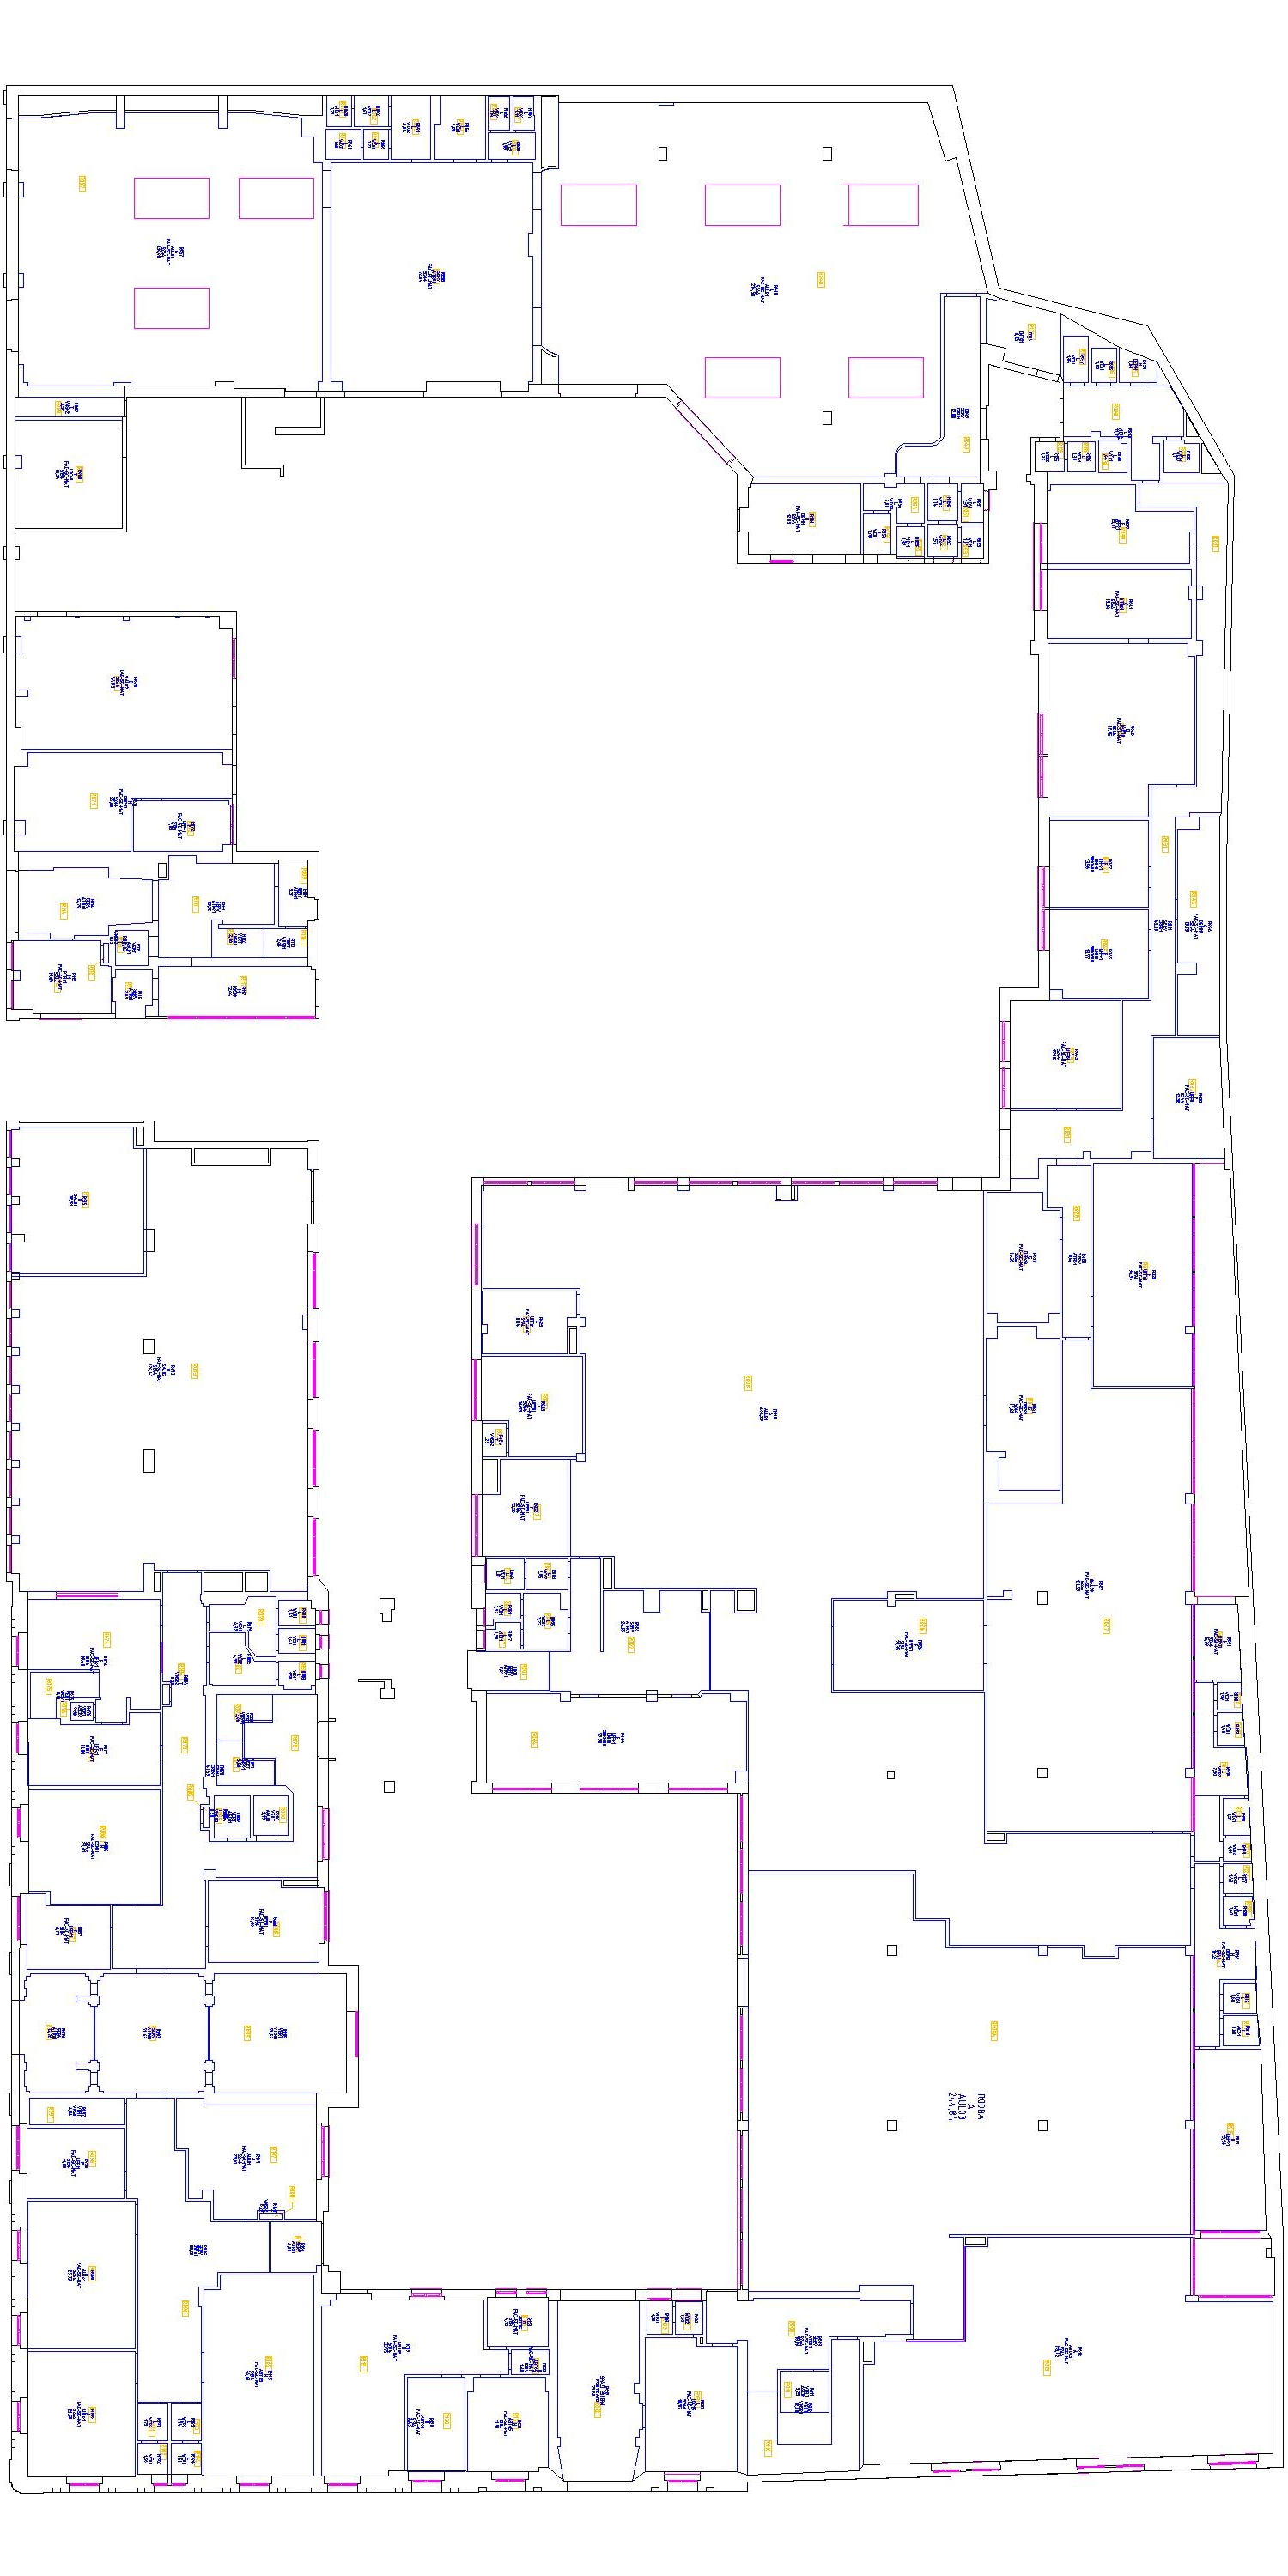
\includegraphics[width=280pt]{Comelico-DXF.jpg}
    \caption{DXF rappresentante il piano rialzato del dipartimento di Informatica}
    \label{fig:Comelico-DXF}
\end{figure}


\begin{figure}[H]
    \centering
    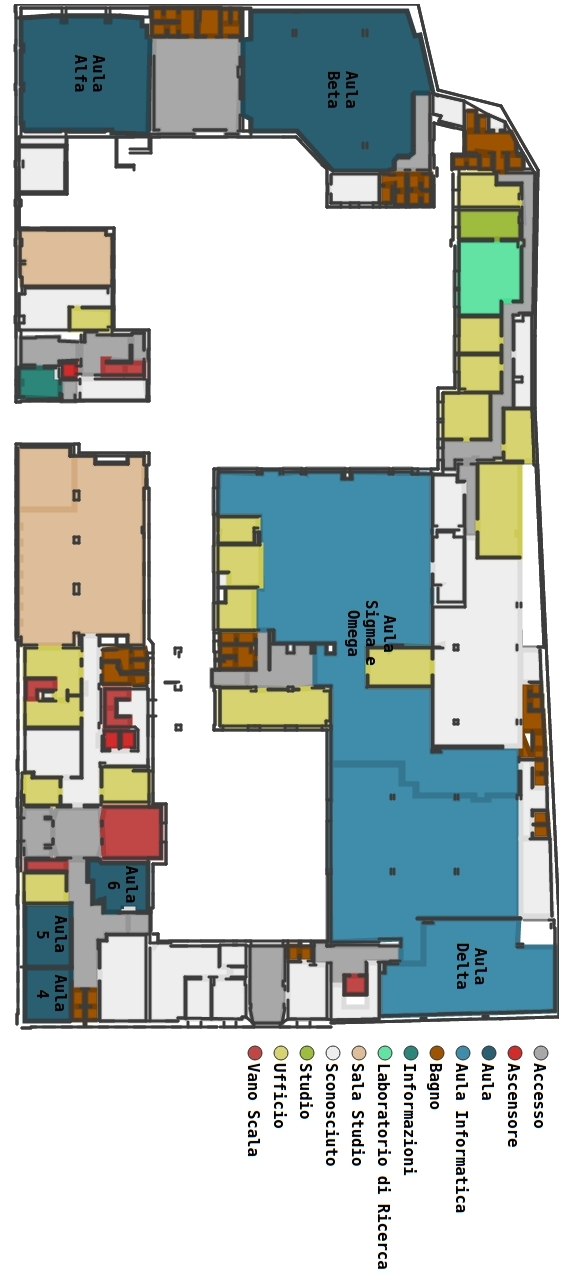
\includegraphics[width=280pt]{Comelico-SVG.jpg}
    \caption{SVG rappresentante il piano rialzato del dipartimento di Informatica}
    \label{fig:Comelico-SVG}
\end{figure}
%PROF: sicuro che sia una buona idea fare vedere questo piano in cui si nota subito non correttezza piatine circa i lavori in aula sigma, tau, e omega?

\newpage
\section{Considerazioni finali sullo sviluppo del progetto e sul miglioramento personale}

Il progetto Spazi-Unimi come detto si proponeva di creare una applicazione multipiattaforma che aiutasse gli utenti ad orientarsi nel contesto dell'Università degli Studi di Milano.
La prima cosa che si può dire giunti alla fine del periodo di tirocinio previsto (18 settimane) è che il progetto è più o meno a metà strada rispetto alla sua conclusione.
Le stime iniziali effettuate dai membri del team prevedevano il completamento del lavoro nei tempi citati quindi si può dire che tali stime non fossero corrette. 
Ben presto infatti ci si è accorti che le problematiche relative allo sviluppo e del sistema erano molto più complesse rispetto alle aspettative iniziali.
Questa sottostima dei tempi è dovuta principalmente alla poca esperienza e soprattutto alla scarsa conoscenza iniziale delle tecnologie e delle tipologie di dati e file con le quali abbiamo dovuto lavorare.

\vspace{5mm} %5mm vertical space

La prima parte del processo di sviluppo del software come detto ha previsto del tempo per la comprensione del linguaggio (Python 3) e della tipologia di database (MongoDB).
In questa fase l'apprendimento è stato molto veloce dato che Python è considerato molto facile da imparare anche grazie alla leggibilità della sua sintassi.
Lo stesso MongoDB è risultato semplice da utilizzare dato che le query e operazioni effettuabili sulle collection del database si possono definire un'estensione di JavaScript.
Superata una certa soglia di apprendimento poi lo sviluppo di nuove funzionalità ha subito una velocizzazione dovuta anche alla possibilità di produrre codice in parallelo, cosa che inizialmente era poco possibile.

\vspace{5mm} %5mm vertical space

Per quanto mi riguarda il processo di integrazione e validazione dei dati forniti dalle due fonti è stato sicuramente il più dispendioso in termini di energie e tempo, ma anche il più interessante.
Le problematicità riscontrate in questa parte del progetto sono dovute per lo più al mancato utilizzo da parte delle fonti di uno standard preciso nella creazione dei file.
Ciò è provocato principalmente dal fatto che le informazioni sono state raccolte in tempi diversi e da persone diverse; in particolare i file DXF essendo in numero molto elevato e risultando elaborati in anni tra loro lontani presentano le problematicità maggiori.  
Ad esempio ciò che ci ha portato a definire un algoritmo di inferenza dei piani è stata la mancata uniformità nello standard di codifica nei nomi proprio dei file DXF.
Questa serie di problemi hanno così allungato molto il tempo di sviluppo della parte back-end togliendo tempo allo sviluppo dell'applicazione vera e propria. %PROF: attenzione: detto così sembrerebbe però che è stato tolto un po' di tempo ma è stato fatto anche il secondo step...

\newpage

La parte del sistema sviluppata però ha una caratteristica su cui ci si è concentrati in maniera prioritaria: il prodotto è affidabile e robusto.
L'affidabilità deriva dall'aver cercato di ottimizzare sempre i dati a nostra disposizione: invece di segnalare le criticità e buttare le informazioni abbiamo analizzato l'informazione cercando di renderla utilizzabile migliorandola.
Come risultato si sono definiti gli algoritmi di controllo presenti in ogni parte del codice che validano e sistemano i dati fornendo un report utile agli utenti che li dovranno aggiornare.
La robustezza invece è stata ottenuta ponendo altri controlli soprattutto in relazione ai file utilizzati come input.  
Inoltre la maggior parte del codice è coperta da test e ciò ci ha portato ad avere una buona sicurezza nel considerare i risultati delle varie elaborazioni come positivi. %PROF: non riesci a quantificare "la maggior parte" con una percentuale? Non dovrebbe essere difficile... non consoco benissimo i tool sotto python ma... probabilmente il package "coverage.py" lo dovrebbe fare...

\vspace{5mm} %5mm vertical space

Un'altra caratteristica fondamentale dei prodotti software che si è cercato di ottimizzare è la qualità del codice.
Python da solo fornisce una sintassi pulita e leggibile ma in molti casi ci si è scontrati con funzioni molto lunghe e complesse che riviste dopo qualche tempo risultavano difficili da comprendere anche a chi le aveva scritte.
Per questo motivo il refactoring è stata una fase fondamentale del nostro processo di sviluppo: ogni qualvolta si notava una porzione di codice da rivedere o lo si faceva immediatamente o si aggiungeva una nota su Trello così da non dimenticarsi della modifica da fare.

Nonostante un team di più persone possa solitamente produrre codice scritto in maniera molto diversa in base al membro impegnato nella scrittura si è cercato di adottare lo stile consigliato di Python\footnote{\url{https://www.python.org/dev/peps/pep-0008}} leggermente adattato per rispecchiare le nostre esigenze.
Un esempio è la denominazione dei metodi privati: tale distinzione in Python non esiste quindi per indicare l'insieme di funzioni che non andrebbero richiamate al di fuori della classe si utilizza un underscore ('\_') prima del nome del metodo.

Sempre con l'obbiettivo della leggibilità del codice scritto si è inoltre aggiunta ad ogni funzione una docstring cioè un commento con il compito di descrizione.
Lo standard utilizzato per tali commenti è stato il seguente:
\begin{itemize}
\item un descrizione veloce del compito della funzione;
\item una lista degli argomenti passati, per ogni argomento viene specificato il tipo previsto e la sua funzione;
\item le specifiche del valore di ritorno della funzione;
\item se necessaria una descrizione più esaustiva e completa delle operazioni svolte in tale procedura. 
\end{itemize}

\vspace{5mm} %5mm vertical space

Per quanto riguarda invece le scelte tecnologiche effettuate all'inizio del progetto, vista la quantità di tempo passata, si possono trarre ora delle conclusioni.

Python 3 si è dimostrato un linguaggio molto potente ed efficace, e grazie all'approccio multi-paradigma ha permesso di implementare sempre il codice nella maniera più semplice ed intuitiva.

\vspace{5mm} %5mm vertical space

MongoDB come database NoSQL si è dimostrato molto utile per quanto riguarda il processo di Data Integration: potendo inserire nella colletion dei documenti aventi strutture diverse non ci si è infatti dovuti preoccupare della miriade di campi 'NULL' che avremmo avuto con un classico database relazionale.

Altro punto a favore di MongoDB sono le query geospaziali molto ben supportate: creando oggetti GeoJson e un indice sui campi che li contengono si possono effettuare facilmente delle richieste particolari legate alle coordinate geografiche; ad esempio è molto facile in questo modo sapere dove ci si trova. %PROF: sicuro? in che senso? segnalare sulla mappa dove ci si trova? Non chiaro in ogni caso

Sempre a proposito degli indici si è cercato di effettuare delle prove per capire quale fosse l'incremento alle prestazioni dovuto al loro utilizzo e quale fosse la struttura migliore per i documenti contenuti nella collection. Le prove su database sono state quattro e si basavano tutte su dei dati fittizi creati grazie alla possibilità di eseguire codice JavaScript sulla console di MongoDB. 
La collection interessata dai test conteneva dati su 1500 edifici aventi ognuno 5 piani in cui vi erano sempre 10 stanze mappate: tale insieme è molto superiore a quello realmente a disposizione, ma è servito per comprendere meglio i tempi di risposta del database.   
Le prove effettuate sono state le seguenti:
\begin{itemize}
\item ricerca di una stanza in una collection con i dati delle aule annidati negli edifici, tempo di calcolo: 5.61 secondi;
\item ricerca di una stanza in una collection contenente una lista di tutte le aule senza annidamento, tempo di calcolo: 12.33 secondi
\item ricerca di una stanza con dati sulle aule annidati negli edifici e con indice creato sui room\_id, tempo di calcolo: 0.17 secondi;
\item ricerca su una collection di aule con indice creato sempre sul room\_id di ogni stanza, tempo di calcolo: 0.15 secondi. 
\end{itemize}

Queste prove hanno dimostrato la validità degli indici in MongoDB e hanno fatto capire che il database si comporta meglio quando i dati sono annidati e non divisi in collection separate.

Ciò ci porta però alla problematica principale emersa dall'utilizzo di MongoDB: effettuando una query in cui ad esempio si specifica un parametro di una stanza da cercare il database ritorna la lista dei documenti rappresentanti gli edifici che contengono almeno un'aula che soddisfa il parametro.
Questo comporta un maggiore spreco di spazio per il fatto di aver ritornato interi documenti e uno spreco di tempo dovuto alla necessità di dover cercare nuovamente le aule interessate all'interno dei documenti ricevuti.
Tale problematica si evidenzia maggiormente in fase di definizione delle API e può essere risolta proprio definendo un'altra collection contenente le informazioni delle aule.  %PROF: può essere risolta... o è stata risolta ?

\vspace{5mm} %5mm vertical space

Dal mio punto di vista lo sviluppo del progetto Spazi-Unimi ha comportato una notevole crescita personale; il fatto di aver imparato, partendo da zero, nuove tecnologie (Python 3, MongoDB, etc.) oltre ad aumentare le mie competenze mi ha fatto comprendere appieno l'importanza in campo informatico di cercare un continuo miglioramento e aggiornamento.

Altra considerazione importante è che questo per me è stato il primo progetto svolto in un team al di fuori dei laboratori didattici fatti durante le lezioni universitarie.
La mancanza di uno sviluppo guidato dall'alto come capita in ambito di insegnamento ha portato a commettere molti errori da parte dei membri del team.
Proprio tali errori e la loro risoluzione (quando possibile) hanno però definito una forte crescita di esperienza.
In molti casi non si è infatti riusciti a mantenere le linee guida dell'XP (Extreme Programming) soprattutto per quanto riguarda il principio KISS (Keep It Simple, Stupid)\footnote{KISS è un principio di design del software che si propone di trovare e implementare la soluzione più semplice del problema.}.
Volendo utilizzare un approccio Big Design Up Front (BDUF)\footnote{Big Design Up Front è un approccio allo sviluppo software che si propone di definire un design completo ed ottimale ancora prima di iniziare a scrivere codice.} in molti casi infatti si è andati a complicare la progettazione e l'implementazione di certe parti del sistema.

Tali errori però sono riconducibili proprio alla mancanza di esperienza dei membri del team e certe volte anche ad una volontà eccessiva di migliorare la qualità del prodotto portandolo così ad una complessità fin troppo elevata in certe sue parti.

\vspace{5mm} %5mm vertical space

A mio modesto parere però il prodotto sin qui sviluppato ha portato alla definizione di un database contenente dati di qualità molto buona che utilizzati nella futura applicazione multi-piattaforma porteranno un notevole beneficio per gli utenti dell'Università degli Studi di Milano.   
%
%

%
%			BIBLIOGRAFIA
%
\nocite{*}
\printbibliography

% 
\end{document}


 
